\chapter{偏微分方程问题}
\label{chap:pde-problems}

一根细棒两端浸在冰水里，中间一段事先被加热过。我们想知道此后每个位置、每个时刻的温度。这个问题的状态不再是有限个数，而是棒上的一整条温度曲线；描述它的方程$\partial_tu=\partial_x^2u$把时间变化率和空间弯曲程度联系起来。

可是只写下这个方程，问题还没有提好。$u=0$、$u=x$、$u=x^2+2t$都满足它，彼此毫无关系。要得到确定的答案，还要说明棒从什么温度开始、两端发生了什么。换成弦的振动，一个初始形状不够，还要知道初始速度；换成水流搬运墨水，只有上游的端点需要提供信息，下游的端点不能随意规定。

数据给对了，还有两件事没有说清。第一，当初始温度带折角、热源有跳跃，或者解在演化中自己长出间断时，“满足方程”这句话是什么意思？第二，方程有了解，解是否唯一？测量误差会不会被放大到毫无意义？

本章在进入具体方程之前把这些问题摆清楚。先把未知场和方程写成统一的形式，再按时间和边界讨论需要什么数据、数据之间要满足什么关系；然后用系数的符号结构区分方程的类型，由此判断信息的传播方式；最后讨论解的几种含义，以及存在、唯一、连续依赖这三个问题怎样依赖于所选的函数空间。后面各章会在具体模型中逐一落实这些条件。

\section{未知场与方程}
\label{sec:pdeprob-fields}

常微分方程的未知量是随时间变化的有限维向量。未知量变成空间上的函数之后，方程要写什么？这种方程和常微分方程有多少相同、从哪里开始不同？

\paragraph{从状态向量到场}
设细棒占据区间$[0,1]$。棒很细，同一截面上的温度可以看成相同，于是在时刻$t$、位置$x$处只有一个温度$u(x,t)$。固定$t$，整条曲线$x\mapsto u(x,t)$就是这一时刻棒的状态。

把棒等分为$N+1$段，步长$h=1/(N+1)$，只记录内部格点$x_j=jh$处的温度，就得到一个$N$维向量，这正是常微分方程意义下的状态。图~\ref{fig:pdeprob-state-to-field}画出同一条温度曲线在两种步长下的采样：格点加密时向量变长，竖线越来越密地铺满曲线下方。

\begin{BookInlineFigure}
  \centering
  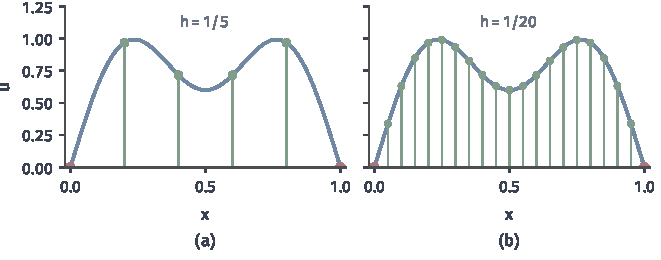
\includegraphics[width=112.0mm]{figures/06-differential-equations/02-partial-differential-equations/matplotlib/pdeprob-state-to-field/figure.pdf}
  \caption{细棒上的温度曲线（蓝）及其格点采样（绿）。曲线为$u=\sin\pi x+0.4\sin3\pi x$，两端值为零（红点）。(a)$h=1/5$，状态是$4$维向量。(b)$h=1/20$，状态是$19$维向量。把步长继续减小，向量就变成整条曲线。}
  \label{fig:pdeprob-state-to-field}
\end{BookInlineFigure}

步长趋于零时，状态不再是有限个数，而是一个函数。这样在空间每一点指定一个量的函数称为\term{场}（field）。每点的量是一个数，就是\term{标量场}（scalar field），如温度、浓度、弦的位移；每点的量是一个向量，就是\term{向量场}（vector field），如流体的速度。

\paragraph{本部分的记号}
从本章开始，空间区域记为开集$\Omega\subset\mathbb{R}^{d}$，边界为$\partial\Omega$，闭包为$\overline{\Omega}$，边界上的单位外法向为$\bm{n}$。空间点写作$\bm{x}$，一维时写作$x$。这里要特别注意：第一部分用$\bm{x}(t)$表示状态，而在这一部分$\bm{x}$只表示位置，状态的角色由整个函数$u(\cdot,t)$担任。

偏导数写作$\partial_tu$、$\partial_xu$、$\partial_{x_i}u$。三个空间微分算子只对$\bm{x}$求导，不涉及$t$，它们是：
\begin{equation}
  \begin{gathered}
    \nabla u=(\partial_{x_1}u,\ldots,\partial_{x_d}u)^{\top},\qquad
    \nabla\cdot\bm{F}=\sum_{i=1}^{d}\partial_{x_i}F_i,\\
    \Delta u=\nabla\cdot(\nabla u)=\sum_{i=1}^{d}\partial_{x_i}^{2}u.
  \end{gathered}
  \label{eq:pdeprob-operators}
\end{equation}
三者分别称为梯度、散度和Laplace算子。这些场运算的定义和计算规则与积分定理配套，可参考\BookChapterRef{chap:integral-theorems}{卷二第27章“积分定理”}。方程中其余各量的写法列在表~\ref{tab:pdeprob-notation}中，后面各章沿用。

\begin{BookInlineTable}
  \centering
  \begin{tabular}{lll}
    \toprule
    记号 & 含义 & 所在位置\\
    \midrule
    $u(\bm{x},t)$ & 未知场 & $\Omega$内 \\
    $f$ & 源项 & $\Omega$内 \\
    $u_0$ & 初值 & $t=0$的$\Omega$上 \\
    $g$ & 边值 & $\partial\Omega$上 \\
    $\bm{A}(\bm{x})$ & 扩散系数矩阵，对称正定 & $\Omega$内 \\
    $\bm{v}(\bm{x},t)$ & 速度场 & $\Omega$内 \\
    $F(u)$ & 依赖于$u$的通量 & 守恒律中 \\
    $H$ & Hamilton量 & Hamilton--Jacobi方程中 \\
    \bottomrule
  \end{tabular}
  \caption{偏微分方程部分的数据记号。}
  \label{tab:pdeprob-notation}
\end{BookInlineTable}

\paragraph{由局部守恒得到方程}
方程的形式并不是约定出来的，它来自物理量的收支。设$u$是某种量的密度，如热量或墨水浓度，$\bm{F}(\bm{x},t)$是通量，表示单位时间穿过单位面积的量，$f$是单位体积内的产生率。任取一块包含在$\Omega$内的小区域$V$，如图~\ref{fig:pdeprob-balance}。$V$内总量的变化率等于流入减去流出，再加上内部产生：
\begin{equation}
  \frac{\mathrm{d}}{\mathrm{d}t}\int_V u\,\mathrm{d}\bm{x}
  =-\int_{\partial V}\bm{F}\cdot\bm{n}\,\mathrm{d}S+\int_V f\,\mathrm{d}\bm{x}.
  \label{eq:pdeprob-balance}
\end{equation}

\begin{BookInlineFigure}
  \centering
  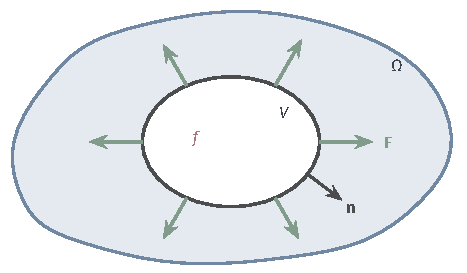
\includegraphics[width=79.1mm]{figures/06-differential-equations/02-partial-differential-equations/tikz/pdeprob-balance/figure.pdf}
  \caption{局部收支。浅蓝区域是$\Omega$，白色小区域$V$内有产生率$f$，绿色箭头表示穿过$\partial V$的通量$\bm{F}$，$\bm{n}$是$\partial V$的单位外法向。$\bm{F}\cdot\bm{n}>0$处量在流出$V$。}
  \label{fig:pdeprob-balance}
\end{BookInlineFigure}

设$u$对$t$连续可微，$\bm{F}$对$\bm{x}$连续可微，$V$的边界足够规则。由散度定理，边界积分可以改写成区域积分，式~\eqref{eq:pdeprob-balance}成为
\[
  \int_V\bigl(\partial_tu+\nabla\cdot\bm{F}-f\bigr)\,\mathrm{d}\bm{x}=0.
\]
这对每个小区域$V$都成立。被积函数连续，若它在某点为正，在该点的一个小球上也为正，取$V$为这个小球就与上式矛盾；为负时同理。所以被积函数处处为零，得到局部形式：
\begin{equation}
  \partial_tu+\nabla\cdot\bm{F}=f.
  \label{eq:pdeprob-conservation}
\end{equation}

式~\eqref{eq:pdeprob-conservation}只有一条关系，却有$u$和$\bm{F}$两个未知对象，还要说明通量怎样由$u$决定。这一步由具体的物理规律给出，不同的规律得到不同的方程。

若热量从高温流向低温，流量正比于温度梯度，就有$\bm{F}=-\bm{A}(\bm{x})\nabla u$，其中对称正定矩阵$\bm{A}$描述材料各方向的导热能力。代入后得到扩散型方程：
\begin{equation}
  \partial_tu-\nabla\cdot\bigl(\bm{A}(\bm{x})\nabla u\bigr)=f.
  \label{eq:pdeprob-diffusion-general}
\end{equation}

若量只是被流体带着走，就有$\bm{F}=\bm{v}u$。由乘积法则，
\[
  \nabla\cdot(\bm{v}u)=\bm{v}\cdot\nabla u+u\,\nabla\cdot\bm{v}.
\]
在不可压缩流动$\nabla\cdot\bm{v}=0$中，第二项消失，方程成为输运形式$\partial_tu+\bm{v}\cdot\nabla u=f$。

若通量是密度自身的函数$F(u)$，例如车流量由车辆密度决定，一维方程就是$\partial_tu+\partial_xF(u)=0$。

弦的振动不是量的收支，而是Newton第二定律。设线密度为$\rho$的弦绷有张力$T$，位移$u(x,t)$和斜率都很小。一小段$[x,x+\delta]$受到两端张力的竖直分力，近似为$T\partial_xu(x+\delta,t)-T\partial_xu(x,t)$，所以
\[
  \rho\,\delta\,\partial_t^{2}u\approx T\bigl(\partial_xu(x+\delta,t)-\partial_xu(x,t)\bigr).
\]
两边除以$\rho\delta$，令$\delta\to0$，并记$c^{2}=T/\rho$，就得到$\partial_t^{2}u=c^{2}\partial_x^{2}u$。

\paragraph{四个模型方程}
取$\bm{A}=\bm{I}$，让演化方程的时间变化率消失，就得到平衡状态的方程。于是我们有四个代表性的方程，它们用同一组变量写成：
\begin{align}
  -\Delta u&=f, \label{eq:pdeprob-poisson}\\
  \partial_tu+\bm{v}\cdot\nabla u&=f, \label{eq:pdeprob-transport}\\
  \partial_tu-\Delta u&=f, \label{eq:pdeprob-heat}\\
  \partial_t^{2}u-c^{2}\Delta u&=f. \label{eq:pdeprob-wave}
\end{align}
依次称为\term{Poisson方程}（Poisson equation）、\term{输运方程}（transport equation）、\term{热方程}（heat equation）和\term{波动方程}（wave equation）。

式~\eqref{eq:pdeprob-poisson}中没有$t$，解只依赖位置，这样的场称为\term{静态场}（stationary field），如稳态温度、膜在固定载荷下的位移。另外三个方程含$t$，解是\term{演化场}（evolving field）。静态问题没有起点，只受区域和边界约束；演化问题的状态从某个时刻出发向前推进，这个差别决定了后面需要什么样的数据。

式~\eqref{eq:pdeprob-heat}和式~\eqref{eq:pdeprob-wave}都含$\Delta u$，要理解这两个方程先要知道$\Delta u$量的是什么。设$u$对$x$三次连续可微，由Taylor展开，
\begin{equation}
  \frac{u(x+h)+u(x-h)}{2}-u(x)=\frac{h^{2}}{2}\partial_x^{2}u(x)+o(h^{2}).
  \label{eq:pdeprob-neighbor-average}
\end{equation}
左边是两个邻点的平均减去当前值。所以$\partial_x^{2}u<0$表示这一点高于邻点的平均，处在凸起上；$\partial_x^{2}u>0$表示这一点低于邻点的平均。

图~\ref{fig:pdeprob-laplace-average}中，红点在峰顶时比两邻点连线的中点高，在山脚时比它低。热方程说温度变化率就是这个差：峰顶降温，山脚升温，形状被抹平。

\begin{BookInlineFigure}
  \centering
  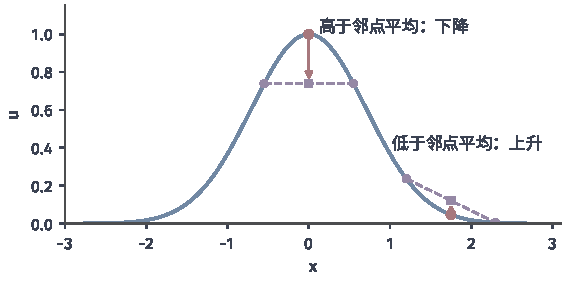
\includegraphics[width=96.0mm]{figures/06-differential-equations/02-partial-differential-equations/matplotlib/pdeprob-laplace-average/figure.pdf}
  \caption{二阶导数比较一点与其邻点的平均。蓝线为$u=\mathrm{e}^{-x^2}$，紫色虚线连接邻点$x_0\pm0.55$，紫色方块是两邻点的平均，红点是$u(x_0)$，红色箭头指示热方程下该点的变化方向。}
  \label{fig:pdeprob-laplace-average}
\end{BookInlineFigure}

在$d$维中，把两个邻点换成以$\bm{x}$为心、半径$r$的球面，同样的Taylor展开给出球面平均减去中心值约等于$\frac{r^{2}}{2d}\Delta u(\bm{x})$。这里用到单位球面上$n_in_j$的平均值，$i=j$时为$1/d$，$i\neq j$时为$0$。$f=0$时这个主项消失；事实上此时两者精确相等，这就是平衡状态下每一点的值等于周围平均的性质。

图~\ref{fig:pdeprob-three-evolutions}把同一个初始鼓包放进三个演化方程。热方程把它压低变宽，输运方程把它原样平移，波动方程把它分成两半向两侧传播。这三种行为分别对应抹平、搬运和分路传播，后面几章会分别加以证明。

\begin{BookInlineFigure}
  \centering
  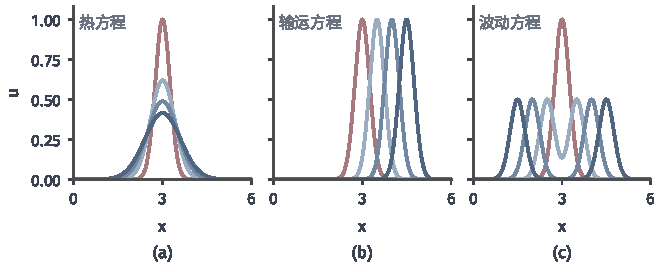
\includegraphics[width=112.0mm]{figures/06-differential-equations/02-partial-differential-equations/matplotlib/pdeprob-three-evolutions/figure.pdf}
  \caption{同一鼓包$u_0(x)=\exp(-(x-3)^2/(2\cdot0.25^2))$在实轴上的演化，红线为$t=0$，蓝色由浅到深为$t=0.5,1,1.5$。(a)$\partial_tu=0.1\,\partial_x^2u$，方差由$0.25^2$增至$0.25^2+0.2t$。(b)$\partial_tu+\partial_xu=0$，解为$u_0(x-t)$。(c)$\partial_t^2u=\partial_x^2u$，初速度为零，解为$\frac12[u_0(x-t)+u_0(x+t)]$。}
  \label{fig:pdeprob-three-evolutions}
\end{BookInlineFigure}

\paragraph{一般形式与线性程度}
上面的方程都是在每一点上把未知函数和它的有限个偏导数联系起来。把静态和演化两种情形放在一起，记自变量为$\bm{z}$：静态问题中$\bm{z}=\bm{x}$，演化问题中$\bm{z}=(\bm{x},t)$。用$D^{k}u$表示$u$的全部$k$阶偏导数。

\begin{definition}[偏微分方程]
\label{def:pdeprob-pde}
设$U$是自变量$\bm{z}$所在的开集，$u:U\to\mathbb{R}$是未知函数。若在$U$的每一点上，$u$及其不超过$m$阶的偏导数满足关系
\begin{equation}
  \mathcal{F}\bigl(\bm{z},u,Du,\ldots,D^{m}u\bigr)=0,
  \label{eq:pdeprob-general-form}
\end{equation}
且$\mathcal{F}$确实依赖某个$m$阶偏导数，则称它是$m$阶\term{偏微分方程}（partial differential equation, PDE）。
\end{definition}

方程按对最高阶导数和$u$的依赖方式分为几个层次，见表~\ref{tab:pdeprob-linearity}。线性方程的系数只依赖$\bm{z}$，算子$L$满足$L(au+bw)=aLu+bLw$；\term{半线性方程}（semilinear equation）的最高阶部分线性，且系数只依赖$\bm{z}$，低阶部分可以非线性；\term{拟线性方程}（quasilinear equation）的最高阶导数仍以一次形式出现，但系数可以依赖$u$和较低阶导数；\term{完全非线性方程}（fully nonlinear equation）对最高阶导数本身非线性。

\begin{BookInlineTable}
  \centering
  \begin{tabular}{lll}
    \toprule
    层次 & 例子 & 判断依据\\
    \midrule
    线性 & $\partial_tu-\nabla\cdot(\bm{A}(\bm{x})\nabla u)=f$ & 系数只依赖$\bm{x}$\\
    半线性 & $\partial_tu-\Delta u=u^{2}$ & 最高阶线性，低阶$u^{2}$\\
    拟线性 & $\partial_tu+u\,\partial_xu=0$ & $\partial_xu$的系数含$u$\\
    完全非线性 & $\partial_tu+\frac12(\partial_xu)^{2}=0$ & 最高阶导数出现平方\\
    \bottomrule
  \end{tabular}
  \caption{偏微分方程按线性程度的层次。}
  \label{tab:pdeprob-linearity}
\end{BookInlineTable}

这些区分影响求解方式。线性方程满足叠加：两个解的线性组合对相应右端仍是解，两个解之差满足右端为零的方程，这是证明唯一性时的基本手段。非线性方程没有这一性质，下面用拟线性方程$\partial_tu+u\,\partial_xu=0$算一个例子。

取两个解$u_1=1$和$u_2=x/(1+t)$。常数$u_1$的两个偏导数都是零，它满足方程。$u_2$的偏导数为
\[
  \partial_tu_2=-\frac{x}{(1+t)^{2}},\qquad
  u_2\,\partial_xu_2=\frac{x}{1+t}\cdot\frac{1}{1+t}=\frac{x}{(1+t)^{2}},
\]
两者相加为零。再看$w=u_1+u_2=1+x/(1+t)$，同样计算得
\[
  \partial_tw+w\,\partial_xw=-\frac{x}{(1+t)^{2}}+\Bigl(1+\frac{x}{1+t}\Bigr)\frac{1}{1+t}=\frac{1}{1+t}\neq0.
\]
两个解之和不是解。

其余几项的作用也可以逐一说清。阶数$m$决定经典意义下解要有几阶导数，也关系到要提供多少数据。系数是常数时，方程在平移下不变，可以用Fourier模式把求导变成乘法；系数随位置变化时这条路不再直接可用。源项$f$让方程非齐次，但在线性问题中可以通过取差消去。

\paragraph{向量未知量}
未知量也可以是向量场。把波动方程降阶就能得到一个例子，做法和常微分方程降阶相同。在一维中记$p=\partial_tu$，$q=\partial_xu$，波动方程$\partial_t^{2}u=c^{2}\partial_x^{2}u$和混合偏导相等分别给出
\[
  \partial_tp=c^{2}\partial_xq,\qquad \partial_tq=\partial_xp.
\]
记$\bm{w}=(p,q)^{\top}$，这是一个一阶方程组：
\begin{equation}
  \partial_t\bm{w}=\bm{B}\,\partial_x\bm{w},\qquad
  \bm{B}=\begin{pmatrix}0&c^{2}\\1&0\end{pmatrix}.
  \label{eq:pdeprob-first-order-system}
\end{equation}
$\bm{B}$的特征值是$\pm c$，恰好是波向两侧传播的速度。降阶用未知量的个数换取了导数的阶数；流体的速度场方程、电磁场方程也是这样的方程组。本部分以标量未知量为主。

\paragraph{函数作为无限维向量}
回到细棒，看空间离散后方程变成什么。在内部格点上用式~\eqref{eq:pdeprob-neighbor-average}近似$\partial_x^{2}u$，并取两端值为零，记$\bm{u}(t)=(u_1(t),\ldots,u_N(t))^{\top}$，热方程成为线性常微分方程组：
\begin{equation}
  \frac{\mathrm{d}\bm{u}}{\mathrm{d}t}=\bm{A}_h\bm{u},\qquad
  (\bm{A}_h\bm{u})_j=\frac{u_{j+1}-2u_j+u_{j-1}}{h^{2}}.
  \label{eq:pdeprob-semi-discrete}
\end{equation}
式中下标超出$1,\ldots,N$的格点值取为零，这样两端的零边值已经写进矩阵。

下面取$N=3$，$h=1/4$，逐项算出这个矩阵的特征值：
\[
  \bm{A}_h=16\begin{pmatrix}-2&1&0\\1&-2&1\\0&1&-2\end{pmatrix}.
\]
$\bm{A}_h$的第$k$个特征向量由$\sin(k\pi x_j)$组成，由和差化积，特征值是
\[
  \lambda_k=-\frac{4}{h^{2}}\sin^{2}\frac{k\pi h}{2},\qquad k=1,\ldots,N.
\]
代入$h=1/4$，得到
\[
  \lambda_1\approx-9.37,\quad \lambda_2=-32,\quad \lambda_3\approx-54.63.
\]

连续问题中对应的等式是
\[
  \partial_x^{2}\sin(k\pi x)=-k^{2}\pi^{2}\sin(k\pi x),
\]
前三个特征值约为$-9.87$、$-39.48$、$-88.83$。向量的分量对应函数在各点的值，矩阵$\bm{A}_h$对应算子$\partial_x^{2}$，特征向量对应正弦模式，矩阵的首末行编码了零边值。

这个类比在一个关键处失效。图~\ref{fig:pdeprob-spectrum-growth}显示，低频特征值随加密趋于$-k^{2}\pi^{2}$，但矩阵的谱范数约为$4/h^{2}$，$N\to\infty$时趋于无穷。

\begin{BookInlineFigure}
  \centering
  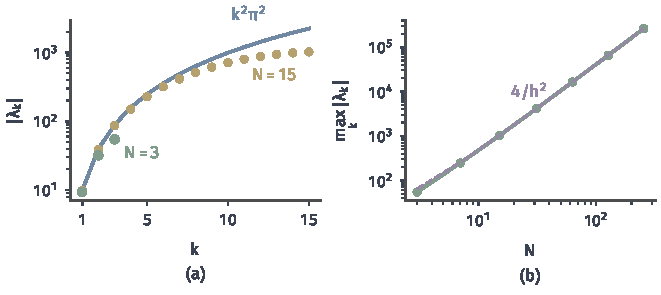
\includegraphics[width=112.0mm]{figures/06-differential-equations/02-partial-differential-equations/matplotlib/pdeprob-spectrum-growth/figure.pdf}
  \caption{式~\eqref{eq:pdeprob-semi-discrete}中矩阵的特征值。(a)第$k$个特征值的绝对值：$N=3$（绿）、$N=15$（黄）、连续问题的$k^2\pi^2$（蓝）。(b)最大特征值绝对值（绿）随$N$的增长，紫色虚线为$4/h^2$。}
  \label{fig:pdeprob-spectrum-growth}
\end{BookInlineFigure}

谱范数正是线性右端的Lipschitz常数。第~\ref{chap:ode-existence-continuation}章的存在性论证依赖右端的Lipschitz条件，而这里的常数随加密无界增长，极限算子$\partial_x^{2}$在$L^{2}(0,1)$或$C[0,1]$这样的空间上不是有界映射：它要消耗两阶导数。所以不能把偏微分方程直接当作无限维常微分方程来套用已有的定理。后面要靠别的结构，例如$\bm{A}_h$的特征值全部为负，来得到估计；这也是为什么必须先说清解和数据所在的空间。

\section{初值与边界数据}
\label{sec:pdeprob-data}

方程只规定区域内部每一点上的局部关系，它本身确定不了解。仍以$(0,1)$上的细棒为例，下面几个函数都满足$\partial_tu=\partial_x^{2}u$：
\[
  u=0,\qquad u=x,\qquad u=x^{2}+2t,\qquad u=\mathrm{e}^{-\pi^{2}t}\sin\pi x.
\]
第三个函数的两个偏导数都是$2$；第四个函数的两个偏导数都等于$-\pi^{2}\mathrm{e}^{-\pi^{2}t}\sin\pi x$。

缺少的信息有多少？一阶常微分方程的通解含一个任意常数，补一个初值就够了。偏微分方程的通解含任意函数。例如$\partial_tu+\partial_xu=0$的解可以写成$u=\varphi(x-t)$，其中$\varphi$是任意可微函数，由链式法则，$\partial_tu=-\varphi'$，$\partial_xu=\varphi'$，两者相加为零。所以需要补充的也是函数，它们定义在比时空低一维的集合上：初始时刻的切片和区域的边界。

演化问题的自变量落在\term{时空柱}（space-time cylinder）$Q=\Omega\times(0,T)$中。图~\ref{fig:pdeprob-cylinder}画出它的三块边界：底面是初始时刻，侧面是空间边界随时间展开，顶面是终止时刻。以热方程为例，典型的问题是
\begin{equation}
  \begin{cases}
    \partial_tu-\Delta u=f & \text{在}\ Q\ \text{内},\\
    u=g & \text{在}\ \partial\Omega\times(0,T)\ \text{上},\\
    u(\cdot,0)=u_0 & \text{在}\ \Omega\ \text{上}.
  \end{cases}
  \label{eq:pdeprob-heat-ibvp}
\end{equation}

\begin{BookInlineFigure}
  \centering
  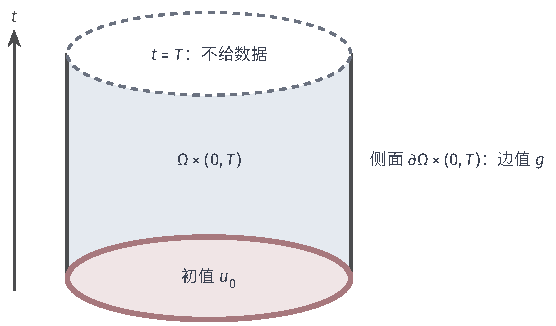
\includegraphics[width=94.1mm]{figures/06-differential-equations/02-partial-differential-equations/tikz/pdeprob-cylinder/figure.pdf}
  \caption{时空柱$Q=\Omega\times(0,T)$。红色底面给初值，深灰色侧面给边值，虚线所示的顶面$t=T$不给数据，那里的值由演化决定。}
  \label{fig:pdeprob-cylinder}
\end{BookInlineFigure}

数据的个数和位置不是随意的，还要与方程传播信息的方式相合。热方程不在顶面给数据，输运方程只在一部分侧面给数据，波动方程在底面要给两个函数。下面分三部分讨论：初始状态要给几个函数、边界上能给什么、两者交接时要满足什么。

\subsection{初始数据}
\label{sec:pdeprob-initial}

为什么热方程只要一个初值，而波动方程要两个？比较这两个方程在$t=0$能告诉我们什么。

\paragraph{时间阶数与初始状态}
在$(0,1)$上给定初始温度$u_0$，且两端为零。热方程的右端可以由$u_0$算出，于是$\partial_tu(\cdot,0)=\partial_x^{2}u_0$，时间一阶导数已经由方程确定，不必再给。

波动方程不同。给定初始位移$u_0$，方程只确定了$\partial_t^{2}u(\cdot,0)=c^{2}\partial_x^{2}u_0$，时间一阶导数还是自由的。这和常微分方程$\ddot{x}=-x$必须同时给位置和速度是一回事，只是位置和速度现在都是函数。所以波动方程的初始状态是一对函数：
\begin{equation}
  u(\cdot,0)=u_0,\qquad \partial_tu(\cdot,0)=u_1.
  \label{eq:pdeprob-wave-initial}
\end{equation}

下面取$c=1$、两端固定，给定同一个初始位移$u_0=\sin\pi x$，算两个不同的解。直接代入可以验证，下面两个函数都满足波动方程和零边值，且在$t=0$的位移都是$\sin\pi x$：
\[
  u^{\mathrm{a}}=\cos(\pi t)\sin\pi x,\qquad
  u^{\mathrm{b}}=\bigl(\cos(\pi t)+\sin(\pi t)\bigr)\sin\pi x.
\]
区别在初始速度：$\partial_tu^{\mathrm{a}}(x,0)=0$，而$\partial_tu^{\mathrm{b}}(x,0)=\pi\sin\pi x$。

图~\ref{fig:pdeprob-wave-velocity}(b)比较弦中点的历史。两条波动曲线从同一点出发，随后分开，所以只给位移不能确定解。同样的初值在热方程下只有一条曲线，就是$\mathrm{e}^{-\pi^{2}t}$，第~\ref{sec:pdeprob-well-posedness}节将证明它是唯一的。

\begin{BookInlineFigure}
  \centering
  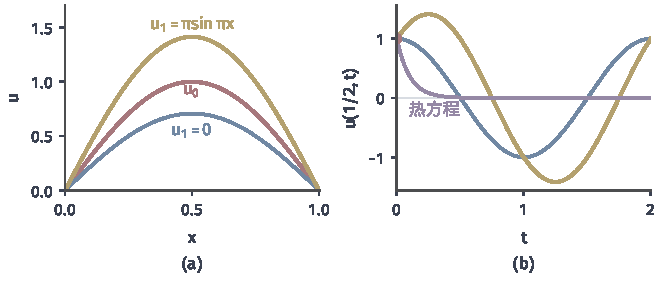
\includegraphics[width=112.0mm]{figures/06-differential-equations/02-partial-differential-equations/matplotlib/pdeprob-wave-velocity/figure.pdf}
  \caption{同一初始位移$u_0=\sin\pi x$（红），$c=1$。(a)$t=1/4$时的弦形：初速度为零（蓝）和初速度为$\pi\sin\pi x$（黄）。(b)中点$x=1/2$的时间历史，蓝、黄同(a)，紫线是热方程在同一初值下的解。}
  \label{fig:pdeprob-wave-velocity}
\end{BookInlineFigure}

一般地，若方程能解出最高阶时间导数，即$\partial_t^{k}u$可以用较低阶时间导数和空间导数表示，就需要$k$个初始函数。这时可以逐阶求出$t=0$处的全部时间导数。以波动方程的$u^{\mathrm{b}}$为例，由初始数据得$\partial_t^{2}u=-\pi^{2}\sin\pi x$，对方程再求一次时间导数得$\partial_t^{3}u=-\pi^{3}\sin\pi x$，这正是$u^{\mathrm{b}}$的Taylor系数。

这个计数只是必要的预期，不保证问题可解。第~\ref{sec:pdeprob-well-posedness}节会看到，把Laplace方程中的一个空间变量当成“时间”，也可以解出二阶导数并给两个初始函数，结果却完全不可用。

\paragraph{初值的光滑程度}
初值的光滑程度决定方程在初始时刻能否按经典意义解释。取折线初值
\begin{equation}
  u_0(x)=\min\{x,1-x\},
  \label{eq:pdeprob-hat}
\end{equation}
它在$x=1/2$处没有导数，$\partial_x^{2}u_0$不存在，所以方程在$t=0$的这一点上没有意义。解决办法是只要求方程在$t>0$成立，初值作为$t\to0$时的极限取到。

这样解释后，热方程和波动方程的表现完全不同。把$u_0$展开成正弦级数，系数为
\[
  b_k=2\int_0^{1}u_0(x)\sin(k\pi x)\,\mathrm{d}x=\frac{4\sin(k\pi/2)}{k^{2}\pi^{2}},
\]
热方程的解和$c=1$的波动方程在初速度为零时的解分别是
\[
  \sum_{k\geq1}b_k\mathrm{e}^{-k^{2}\pi^{2}t}\sin k\pi x,\qquad
  \sum_{k\geq1}b_k\cos(k\pi t)\sin k\pi x.
\]

对热方程，每求一次$x$的导数系数多一个因子$k\pi$，但只要$t>0$，因子$\mathrm{e}^{-k^{2}\pi^{2}t}$比任何多项式衰减得都快，求导后的级数仍然收敛，解立即变得光滑。在$t=0$，二阶导数的级数通项是$-4\sin(k\pi/2)\sin(k\pi x)$，不趋于零，这正对应$\partial_x^{2}u_0$不存在。

对波动方程，系数没有衰减因子。解等于$\frac12[u_0^{*}(x-t)+u_0^{*}(x+t)]$，其中$u_0^{*}$是$u_0$在实轴上的奇周期延拓。折角被原样带着走，分成两个折角向两边移动。图~\ref{fig:pdeprob-kink-heat-wave}对比了两种情形：(a)的折角瞬间变圆，(b)的折角一直保持。所以波动方程在$t>0$时沿这两条线仍不能按经典意义解释；这样的函数算不算解，要到第~\ref{sec:pdeprob-solutions}节再回答。

\begin{BookInlineFigure}
  \centering
  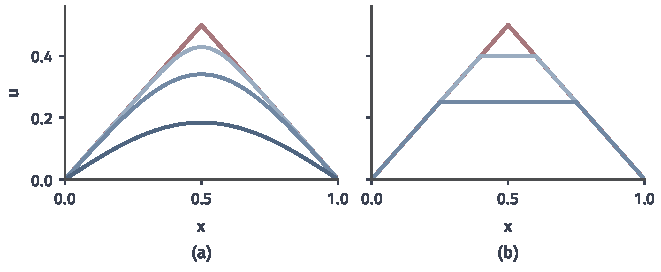
\includegraphics[width=112.0mm]{figures/06-differential-equations/02-partial-differential-equations/matplotlib/pdeprob-kink-heat-wave/figure.pdf}
  \caption{折线初值$u_0=\min\{x,1-x\}$（红），两端为零。(a)热方程，蓝色由浅到深为$t=0.004,0.02,0.08$，折角立即消失（$600$项正弦级数）。(b)波动方程，$c=1$，初速度为零，蓝色由浅到深为$t=0.1,0.25$，两个折角分别向左右移动，中间是一段平台。}
  \label{fig:pdeprob-kink-heat-wave}
\end{BookInlineFigure}

\subsection{边界数据}
\label{sec:pdeprob-boundary}

区域有边界，边界上发生的事也要交代。边界条件规定的可以是场值，可以是穿过边界的通量，也可以是两者之间的关系。

\paragraph{三类边界条件}
记$\partial_{\bm{n}}u=\nabla u\cdot\bm{n}$，它是$u$沿离开区域方向的变化率，称为\term{法向导数}（normal derivative）。按照热传导的语言，$\partial\Omega$上常见的条件是：
\begin{align}
  u&=g, \label{eq:pdeprob-dirichlet}\\
  \partial_{\bm{n}}u&=g, \label{eq:pdeprob-neumann}\\
  \partial_{\bm{n}}u+\alpha u&=g. \label{eq:pdeprob-robin}
\end{align}
依次称为\term{Dirichlet边界条件}（Dirichlet boundary condition）、\term{Neumann边界条件}（Neumann boundary condition）和\term{Robin边界条件}（Robin boundary condition）。

Dirichlet条件直接规定温度，如棒端浸在恒温水中。Neumann条件规定穿过边界的通量，向外的热流是$-\partial_{\bm{n}}u$，所以$g=0$表示绝热。Robin条件来自Newton冷却定律：向外的热流正比于边界温度与环境温度$u_{\mathrm{env}}$之差，$-\partial_{\bm{n}}u=\alpha(u-u_{\mathrm{env}})$，整理后就是式~\eqref{eq:pdeprob-robin}，其中$g=\alpha u_{\mathrm{env}}$。

物理上$\alpha\geq0$。$\alpha<0$意味着边界越热吸收得越多，这种正反馈下后面的估计不再成立。系数不是单位矩阵时，通量是$\bm{A}\nabla u$，法向导数相应换成$\bm{n}^{\top}\bm{A}\nabla u$。不同边界段可以使用不同类型，如图~\ref{fig:pdeprob-boundary-types}。

\begin{BookInlineFigure}
  \centering
  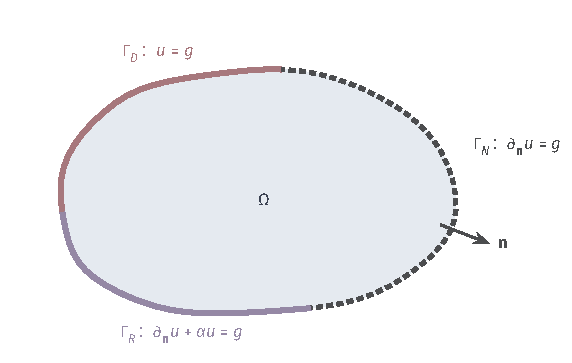
\includegraphics[width=96.9mm]{figures/06-differential-equations/02-partial-differential-equations/tikz/pdeprob-boundary-types/figure.pdf}
  \caption{同一区域的边界分成三段：红色段$\Gamma_D$规定场值，深灰虚线段$\Gamma_N$规定法向导数，紫色段$\Gamma_R$规定场值和法向导数的组合。$\bm{n}$是单位外法向。}
  \label{fig:pdeprob-boundary-types}
\end{BookInlineFigure}

边界类型会改变解本身。下面在$(0,1)$上取方程$-u''=2$和右端条件$u(1)=0$，通解是
\[
  u(x)=-x^{2}+Ax+B.
\]
左端点的外法向指向$-x$方向，所以左端的$\partial_{\bm{n}}u=-u'(0)$。下面依次取三种条件。

Dirichlet条件$u(0)=0$给出$B=0$，再由$u(1)=0$得$A=1$，于是
\[
  u(x)=x(1-x),\qquad \max_xu=\frac14.
\]

Neumann条件$u'(0)=0$给出$A=0$，再由$u(1)=0$得$B=1$，于是
\[
  u(x)=1-x^{2},\qquad \max_xu=1.
\]

Robin条件取$\alpha=1$、$g=0$，即$-u'(0)+u(0)=0$，给出$A=B$。再由$u(1)=-1+2B=0$得$B=1/2$，于是
\[
  u(x)=\frac12+\frac12x-x^{2},\qquad \max_xu=u\Bigl(\frac14\Bigr)=\frac{9}{16}.
\]

图~\ref{fig:pdeprob-bc-solutions}中，三条曲线的热源和右端相同，只有左端不同：Dirichlet曲线被钉在零，Neumann曲线的切线水平，Robin曲线的切线斜率等于端点值$1/2$。左端越容易散热，整根棒越凉：Dirichlet、Robin、Neumann三种情形的最高温依次是$1/4$、$9/16$、$1$。

\begin{BookInlineFigure}
  \centering
  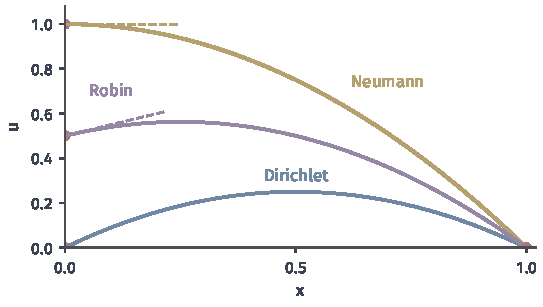
\includegraphics[width=92.0mm]{figures/06-differential-equations/02-partial-differential-equations/matplotlib/pdeprob-bc-solutions/figure.pdf}
  \caption{$-u''=2$、$u(1)=0$在三种左端条件下的解。红点是端点值，虚线是左端切线。}
  \label{fig:pdeprob-bc-solutions}
\end{BookInlineFigure}

\paragraph{输运方程的入流边界}
对$\Omega$的整个边界都规定数据，在二阶椭圆方程中是合理的，在输运方程中却不行。想象水流搬运墨水：墨水的浓度由上游决定，下游端点流出的是已经确定的东西，不能再规定。

在$(0,1)$上取$v=1$，方程$\partial_tu+\partial_xu=0$的信息沿直线$x=x_0+t$传递。设$u(\cdot,0)=u_0$，左端$u(0,t)=g(t)$，沿着这些路径回溯，解是
\begin{equation}
  u(x,t)=\begin{cases}u_0(x-t),&x>t,\\ g(t-x),&x<t.\end{cases}
  \label{eq:pdeprob-transport-solution}
\end{equation}
右端的值$u(1,t)$已经由式~\eqref{eq:pdeprob-transport-solution}确定。若再独立规定$u(1,t)=h(t)$，除非$h$恰好等于算出来的值，否则问题无解。

一般地，定义\term{入流边界}（inflow boundary）和\term{出流边界}（outflow boundary）为
\begin{equation}
  \Gamma_{-}=\{\bm{x}\in\partial\Omega:\bm{v}\cdot\bm{n}<0\},\qquad
  \Gamma_{+}=\{\bm{x}\in\partial\Omega:\bm{v}\cdot\bm{n}>0\}.
  \label{eq:pdeprob-inflow}
\end{equation}
$\bm{v}\cdot\bm{n}<0$表示流动指向区域内部，边界数据只在$\Gamma_{-}$上给出；$\bm{v}$随时间变化时，这两部分也随时间变化。入流边界的位置由速度场决定，而不是由几何形状决定。

图~\ref{fig:pdeprob-inflow}画出区间上的三个速度场。(a)$v=1$，只有左端入流。(b)$v=x-1/2$，两端的外法向分别与速度同向，都是出流，因此端点不需要任何数据，解完全由初值决定。(c)$v=1/2-x$，两端都是入流，都要给数据。

\begin{BookInlineFigure}
  \centering
  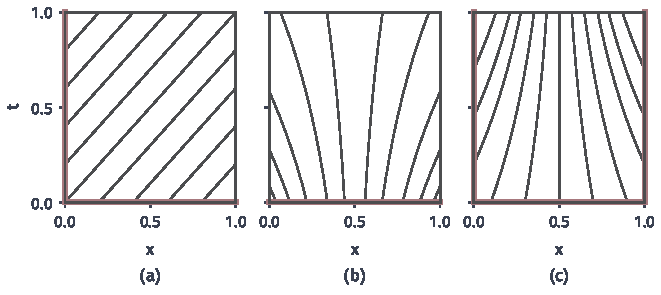
\includegraphics[width=112.0mm]{figures/06-differential-equations/02-partial-differential-equations/matplotlib/pdeprob-inflow/figure.pdf}
  \caption{区间$(0,1)$上三个速度场的粒子路径$\mathrm{d}x/\mathrm{d}t=v$（深灰），红色粗线是需要给数据的边界。(a)$v=1$。(b)$v=x-\frac12$，两端都是出流。(c)$v=\frac12-x$，两端都是入流。每条路径都从红线出发。}
  \label{fig:pdeprob-inflow}
\end{BookInlineFigure}

只在入流边界给数据为什么足够？设$\nabla\cdot\bm{v}=0$，$u$是光滑解，$f=0$。将方程乘以$u$并在$\Omega$上积分。由$\nabla\cdot\bm{v}=0$，对流项可以写成散度：
\[
  u\,\bm{v}\cdot\nabla u=\frac12\nabla\cdot(\bm{v}u^{2}).
\]
再由散度定理，得到
\begin{equation}
  \frac{\mathrm{d}}{\mathrm{d}t}\frac12\int_\Omega u^{2}\,\mathrm{d}\bm{x}
  =-\frac12\int_{\partial\Omega}(\bm{v}\cdot\bm{n})\,u^{2}\,\mathrm{d}S.
  \label{eq:pdeprob-transport-energy}
\end{equation}
出流边界上$\bm{v}\cdot\bm{n}>0$，这一项只会减少能量，不需要控制；入流边界上这一项会增加能量，必须由数据控制。若两个解的初值相同、入流数据相同，它们之差$w$满足式~\eqref{eq:pdeprob-transport-energy}，且$\Gamma_{-}$上$w=0$，所以$\int_\Omega w^{2}$不增，从零出发恒为零。入流数据恰好足以确定解。

\subsection{数据相容性}
\label{sec:pdeprob-compatibility}

初值和边值是分别给出的，但它们在角点处相遇；有些问题的数据之间还有整体的约束。给的数据多，并不意味着有解。

\paragraph{角点处的相容条件}
回到$(0,1)$上的细棒。若初始温度处处为$1$，两端却保持为$0$，那么在角点$(x,t)=(0,0)$附近，沿$t=0$趋近得到$1$，沿$x=0$趋近得到$0$，解不可能在角点连续。

要让解在$\overline{Q}$上连续，需要初值在边界上的取值和边值在初始时刻一致，即零阶\term{相容条件}（compatibility condition）：
\begin{equation}
  u_0(\bm{x})=g(\bm{x},0),\qquad \bm{x}\in\partial\Omega.
  \label{eq:pdeprob-compat-zero}
\end{equation}

要求解更光滑时条件也更多。假设$u$在角点附近有连续的$\partial_tu$和$\partial_x^{2}u$，在左端$x=0$上有$u(0,t)=g(t)$，对$t$求导得$\partial_tu(0,t)=g'(t)$。令$t\to0$，再利用热方程$\partial_tu=\partial_x^{2}u+f$，就得到一阶相容条件：
\begin{equation}
  g'(0)=u_0''(0)+f(0,0).
  \label{eq:pdeprob-compat-one}
\end{equation}
式~\eqref{eq:pdeprob-compat-one}不是额外的物理假设，只是方程在角点处的推论。若要求解有更高阶的连续导数，同样的步骤可以继续，每多要求一阶时间导数，就多一个条件。波动方程的情形类似，表~\ref{tab:pdeprob-compatibility}列出左端点的前几个条件，其中$g$是左端的边值。

\begin{BookInlineTable}
  \centering
  \begin{tabular}{lll}
    \toprule
    方程 & 希望连续到角点的量 & 相容条件\\
    \midrule
    热方程 & $u$ & $u_0(0)=g(0)$\\
    热方程 & $u,\partial_tu,\partial_x^{2}u$ & 另加$g'(0)=u_0''(0)+f(0,0)$\\
    波动方程 & $u$ & $u_0(0)=g(0)$\\
    波动方程 & $u,\partial_tu$ & 另加$u_1(0)=g'(0)$\\
    波动方程 & 全部二阶导数 & 另加$g''(0)=c^{2}u_0''(0)+f(0,0)$\\
    \bottomrule
  \end{tabular}
  \caption{角点处的相容条件随所要求的光滑程度增加。}
  \label{tab:pdeprob-compatibility}
\end{BookInlineTable}

相容条件不满足时，问题不一定无解，而是解的光滑性受限，受限的方式随方程而不同。图~\ref{fig:pdeprob-corner-mismatch}比较初值为$1$、边值为$0$时的两种情形。(a)热方程的解在$t>0$时光滑，不连续性只局限在角点。(b)输运方程的解由式~\eqref{eq:pdeprob-transport-solution}给出，在直线$x=t$左侧为$0$、右侧为$1$，角点处的矛盾被带进区域内部，变成一条持续的间断线。

\begin{BookInlineFigure}
  \centering
  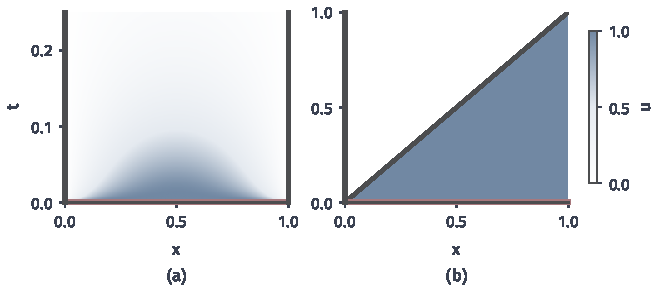
\includegraphics[width=112.0mm]{figures/06-differential-equations/02-partial-differential-equations/matplotlib/pdeprob-corner-mismatch/figure.pdf}
  \caption{初值$u_0=1$（红线）与边值$0$（深灰竖线）不相容。颜色表示$u$的值。(a)热方程，由奇数项正弦级数$\sum_{k}\frac{4}{k\pi}\mathrm{e}^{-k^2\pi^2t}\sin k\pi x$计算。(b)输运方程$v=1$，深灰斜线是间断线$x=t$。两图的时间范围不同。}
  \label{fig:pdeprob-corner-mismatch}
\end{BookInlineFigure}

\paragraph{整体的积分约束}
相容不只发生在角点。考虑Poisson方程配Neumann条件：
\begin{equation}
  -\Delta u=f\ \ \text{在}\ \Omega\ \text{内},\qquad
  \partial_{\bm{n}}u=g\ \ \text{在}\ \partial\Omega\ \text{上},
  \label{eq:pdeprob-neumann-problem}
\end{equation}
其中$\Omega$有界，边界足够规则。把方程在$\Omega$上积分，由散度定理，
\[
  \int_\Omega\Delta u\,\mathrm{d}\bm{x}=\int_{\partial\Omega}\partial_{\bm{n}}u\,\mathrm{d}S.
\]
于是若解存在，数据必须满足
\begin{equation}
  \int_\Omega f\,\mathrm{d}\bm{x}+\int_{\partial\Omega}g\,\mathrm{d}S=0.
  \label{eq:pdeprob-neumann-compat}
\end{equation}

这个条件的含义是收支平衡。$\int f$是内部的总产热，$\int g=\int\partial_{\bm{n}}u$是从外部流入的总热量，平衡状态要求两者之和为零。一个绝热的棒内部持续加热，不可能达到稳态。

在$(0,1)$上取$f=1$、两端绝热$u'(0)=u'(1)=0$。式~\eqref{eq:pdeprob-neumann-compat}左边是$1\neq0$，方程$-u''=1$无解。对应的演化问题$\partial_tu=\partial_x^{2}u+1$却有解，例如从$u_0=\frac12\cos\pi x$出发，
\[
  u(x,t)=t+\frac12\mathrm{e}^{-\pi^{2}t}\cos\pi x.
\]
图~\ref{fig:pdeprob-neumann-balance}(a)中，形状的起伏很快消失，而整体温度以速度$1$不断上升，没有稳态可趋近。

现在改为边界散热，取$u'(0)=1/2$，$u'(1)=-1/2$。这时$\partial_{\bm{n}}u$在两端都是$-1/2$，式~\eqref{eq:pdeprob-neumann-compat}左边是$1-\frac12-\frac12=0$。逐次积分得到解
\[
  u(x)=-\frac{x^{2}}{2}+\frac{x}{2}+C,
\]
其中$C$是任意常数，如图~\ref{fig:pdeprob-neumann-balance}(b)。约束满足了，解却不唯一：方程和边界条件都只含$u$的导数，看不到整体平移。

\begin{BookInlineFigure}
  \centering
  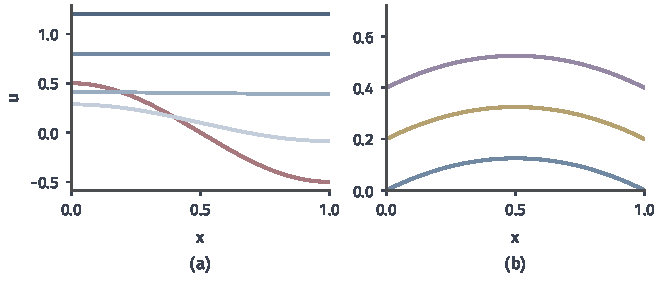
\includegraphics[width=112.0mm]{figures/06-differential-equations/02-partial-differential-equations/matplotlib/pdeprob-neumann-balance/figure.pdf}
  \caption{Neumann问题的积分约束。(a)绝热棒内持续加热，初值（红）的起伏消失，整体上升，蓝色由浅到深为$t=0.1,0.4,0.8,1.2$。(b)加热与散热平衡时$-u''=1$的解$-x^2/2+x/2+C$，$C=0,0.2,0.4$，彼此只差常数。}
  \label{fig:pdeprob-neumann-balance}
\end{BookInlineFigure}

这和线性方程组完全相同。把棒分成三段，每段写热量收支，绝热端没有通量，得到系数矩阵
\[
  \bm{B}=\begin{pmatrix}1&-1&0\\-1&2&-1\\0&-1&1\end{pmatrix},
  \qquad \bm{B}\bm{1}=\bm{0},\qquad \bm{1}^{\top}\bm{B}=\bm{0}^{\top},
\]
其中$\bm{1}=(1,1,1)^{\top}$。方程$\bm{B}\bm{u}=\bm{b}$有解当且仅当$\bm{1}^{\top}\bm{b}=0$，有解时解差$\bm{1}$的倍数。积分约束对应对$\bm{1}$的正交条件，任意常数对应零空间。

这些例子说明，不能靠增加数据的数量来保证有解。数据太少时解不唯一，例如区间上$-u''=f$只给一个端点；数据太多时互相冲突，例如输运方程同时规定两端；个数恰好，也可能违反积分约束。判断的依据是方程的传播方式和结构，下一节把这件事说清楚。

\section{方程类型}
\label{sec:pdeprob-types}

Poisson方程、热方程和波动方程都是二阶线性方程，需要的数据却不同，传播信息的方式也不同。能否不解方程，只看系数就把它们区分开？

\paragraph{主部与高频响应}
记自变量为$\bm{z}\in\mathbb{R}^{N}$，二阶线性方程写成
\begin{equation}
  \sum_{i,j=1}^{N}M_{i,j}(\bm{z})\,\partial_{z_i}\partial_{z_j}u+(\text{一阶及零阶项})=f,
  \label{eq:pdeprob-second-order}
\end{equation}
其中$\bm{M}(\bm{z})$是实对称矩阵。对称性不是限制：混合偏导相等，$M_{i,j}$与$M_{j,i}$只有两者之和起作用，可以都换成平均值。二阶项的全体称为方程的\term{主部}（principal part）。

为什么分类只看主部？在一点附近把系数看成常数，代入高频振荡$u=\mathrm{e}^{\mathrm{i}\bm{\xi}\cdot\bm{z}}$。二阶项给出因子$-\bm{\xi}^{\top}\bm{M}\bm{\xi}$，大小与$\lVert\bm{\xi}\rVert_2^{2}$同阶，一阶项只有$\lVert\bm{\xi}\rVert_2$的量级。频率越高，主部越占支配地位。

所以方程对高频振荡的反应由二次型$\bm{\xi}^{\top}\bm{M}\bm{\xi}$决定。若对所有非零$\bm{\xi}$它都不为零，任何方向的高频振荡都会被主部放大成很大的量，无法存在于解中，除非右端也这样振荡；若沿某个方向它等于零，主部感觉不到沿这个方向的振荡，这种振荡就可以在解中传播。二次型的性质由$\bm{M}$的特征值的符号决定。

\begin{definition}[二阶线性方程的类型]
\label{def:pdeprob-types}
设$\bm{M}(\bm{z})$是式~\eqref{eq:pdeprob-second-order}在点$\bm{z}$处的系数矩阵。根据它的特征值，称方程在该点是
\begin{enumerate}
  \item \term{椭圆型}（elliptic）：全部特征值非零且同号；
  \item \term{抛物型}（parabolic）：恰有一个特征值为零，其余同号，且相应零特征方向上有一阶项；
  \item \term{双曲型}（hyperbolic）：全部特征值非零，且恰有一个的符号与其余相反。
\end{enumerate}
\end{definition}

这三类并不穷尽所有情形。$N\geq4$时可以有两正两负的特征值，例如下面的方程不属于这三类：
\[
  \partial_{z_1}^{2}u+\partial_{z_2}^{2}u-\partial_{z_3}^{2}u-\partial_{z_4}^{2}u=0.
\]

抛物型的定义中要求一阶项，是因为把$\partial_x^{2}u=0$看成$(x,t)$的方程时，$\bm{M}$也有零特征值，但其中$t$只是参数，方程实质上是关于$x$的常微分方程。

把四个模型代入。Poisson方程的$\bm{z}=\bm{x}$，$\bm{M}=-\bm{I}$，椭圆型。热方程的$\bm{z}=(\bm{x},t)$，
\[
  \bm{M}=\operatorname{diag}(-1,\ldots,-1,0),
\]
零特征方向是时间方向，那里有一阶项$\partial_tu$，抛物型。波动方程的$\bm{z}=(\bm{x},t)$，
\[
  \bm{M}=\operatorname{diag}(-c^{2},\ldots,-c^{2},1),
\]
恰有一个特征值与其余反号，双曲型。输运方程是一阶方程，没有二阶项，不在这个分类中。

两个变量时分类有一个常用的判别式。考虑方程
\[
  a_1\partial_y^{2}u+2a_2\partial_y\partial_zu+a_3\partial_z^{2}u+(\text{低阶项})=f.
\]
它的系数矩阵的行列式是$a_1a_3-a_2^{2}$，也就是两个特征值之积。于是$a_2^{2}-a_1a_3$小于零、等于零、大于零分别对应椭圆、抛物、双曲型（抛物型另需一阶项）。

名称来自把$\partial_x$换成$\xi$、把$\partial_t$换成$\tau$后得到的曲线，如图~\ref{fig:pdeprob-conics}：二维Laplace算子给出$\xi^{2}+\tau^{2}=1$，热算子给出$\tau=\xi^{2}$，波动算子给出$\tau^{2}-\xi^{2}=1$。这只解释了名字的来历，真正起作用的是下面要讲的传播方式。

\begin{BookInlineFigure}
  \centering
  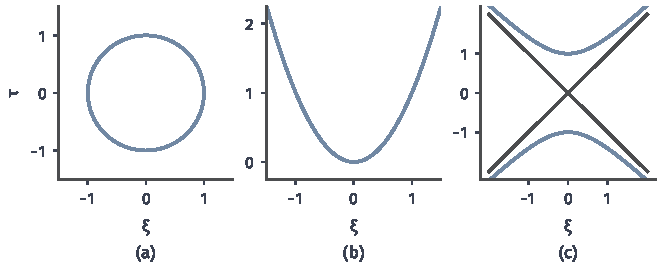
\includegraphics[width=112.0mm]{figures/06-differential-equations/02-partial-differential-equations/matplotlib/pdeprob-conics/figure.pdf}
  \caption{三类方程名称的来历。(a)椭圆$\xi^2+\tau^2=1$。(b)抛物线$\tau=\xi^2$。(c)双曲线$\tau^2-\xi^2=1$，深灰直线是渐近线$\tau=\pm\xi$，它们对应二次型为零的方向。}
  \label{fig:pdeprob-conics}
\end{BookInlineFigure}

\paragraph{分类不依赖坐标}
类型只有在换坐标后不变才有意义。下面的引理说明它只依赖特征值符号的个数。

\begin{lemma}[类型在坐标变换下不变]
\label{lem:pdeprob-invariance}
设$\bm{y}=\bm{\Phi}(\bm{z})$是二阶连续可微的可逆坐标变换，其Jacobi矩阵$\bm{J}$处处可逆。在新坐标下，式~\eqref{eq:pdeprob-second-order}的系数矩阵是
\begin{equation}
  \widetilde{\bm{M}}=\bm{J}\bm{M}\bm{J}^{\top},
  \label{eq:pdeprob-congruence}
\end{equation}
且$\widetilde{\bm{M}}$与$\bm{M}$的正、负、零特征值个数分别相同。
\end{lemma}

\begin{proof}
记$\widetilde{u}(\bm{y})=u(\bm{z})$。由链式法则，
\[
  \partial_{z_i}u=\sum_{k}J_{k,i}\,\partial_{y_k}\widetilde{u}.
\]
再求一次导数，二阶导数项来自对$\partial_{y_k}\widetilde{u}$求导，对$J_{k,i}$求导只产生一阶项，于是
\[
  \partial_{z_i}\partial_{z_j}u=\sum_{k,l}J_{k,i}J_{l,j}\,\partial_{y_k}\partial_{y_l}\widetilde{u}+(\text{一阶项}).
\]
代入式~\eqref{eq:pdeprob-second-order}，$\partial_{y_k}\partial_{y_l}\widetilde{u}$的系数是$\sum_{i,j}J_{k,i}M_{i,j}J_{l,j}$，这就是式~\eqref{eq:pdeprob-congruence}。

$\bm{M}$的正特征值个数等于使二次型在其上正定的子空间的最大维数。变量替换$\bm{\xi}=\bm{J}^{\top}\bm{\eta}$是线性双射，把$\bm{M}$的这类子空间一一映成$\widetilde{\bm{M}}$的这类子空间，维数不变。负特征值同理，零特征值的个数由总数$N$确定。
\end{proof}

\paragraph{特征方向}
引理还回答了哪些曲面特殊。设曲面由$\varphi(\bm{z})=$常数给出，$\nabla_{\bm{z}}\varphi\neq\bm{0}$。若把$\varphi$取作新坐标$y_1$，$\bm{J}$的第一行就是$(\nabla_{\bm{z}}\varphi)^{\top}$，由式~\eqref{eq:pdeprob-congruence}，
\[
  \widetilde{M}_{1,1}=(\nabla_{\bm{z}}\varphi)^{\top}\bm{M}\,\nabla_{\bm{z}}\varphi.
\]
若这个量为零，新方程中不含$\partial_{y_1}^{2}\widetilde{u}$，方程就无法用曲面上的值和一阶法向导数算出二阶法向导数。这样的曲面称为\term{特征曲面}（characteristic surface），两个自变量时称为\term{特征线}（characteristic curve）。二阶法向导数穿过它可以有跳跃，解的不光滑性可以沿它存在。

下面用一个可以手算的方程走一遍。考虑
\[
  \partial_y^{2}u+4\partial_y\partial_zu+3\partial_z^{2}u=0.
\]
这里$a_1=1$，$a_2=2$，$a_3=3$，判别式$a_2^{2}-a_1a_3=1>0$，方程是双曲型。系数矩阵的两个特征值是$2\pm\sqrt{5}$，确实异号。

把算子分解为两个一阶因子，
\[
  \partial_y^{2}+4\partial_y\partial_z+3\partial_z^{2}=(\partial_y+\partial_z)(\partial_y+3\partial_z).
\]
第一个因子把任何$\psi(y-z)$变成零，第二个因子把任何$\varphi(3y-z)$变成零，因此方程的通解是
\[
  u(y,z)=\varphi(3y-z)+\psi(y-z).
\]
验证特征条件：取$\varphi_1=y-z$，梯度$(1,-1)^{\top}$代入二次型得$1-4+3=0$；取$\varphi_2=3y-z$，梯度$(3,-1)^{\top}$代入得$9-12+3=0$。解确实由沿这两族直线传播的两个函数组成。

三个模型的特征曲面反映了各自的传播方式。对Poisson方程，$\bm{M}=-\bm{I}$，二次型只在零向量上为零，没有特征曲面。对热方程，$\nabla\varphi$必须只有时间分量，特征曲面是水平的$t=$常数。对一维波动方程，二次型$\tau^{2}-c^{2}\xi^{2}$的零点给出直线$x\pm ct=$常数。

\paragraph{类型决定传播方式}
图~\ref{fig:pdeprob-dependence}用一个内部点$P$说明三种类型的依赖关系。椭圆型中，$P$处的值受整个边界影响，没有时间方向，也没有“上游”。抛物型中，$P$处的值依赖此前全部时刻的整个区域；特征面水平，信息在同一时刻立刻到达各处。双曲型中，$P$处的值只依赖向过去张开的一个圆锥。

\begin{BookInlineFigure}
  \centering
  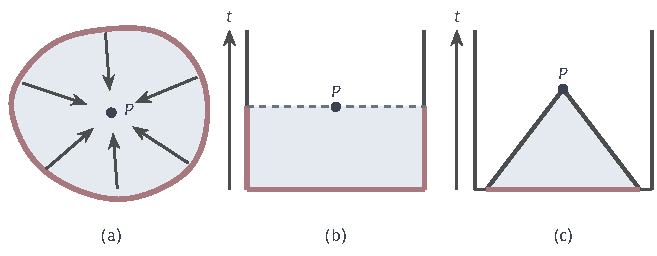
\includegraphics[width=111.3mm]{figures/06-differential-equations/02-partial-differential-equations/tikz/pdeprob-dependence/figure.pdf}
  \caption{内部点$P$的值依赖哪些数据（红）。(a)椭圆型：整个边界都影响$P$。(b)抛物型：时空图中，$P$之前的全部初值和侧面边值都影响$P$，浅蓝部分为依赖区域。(c)双曲型：只有深灰特征线所夹的底边影响$P$，这段红色底边之外的初值不起作用。}
  \label{fig:pdeprob-dependence}
\end{BookInlineFigure}

用点刺激可以把这种差别算出来。把总量为$1$的源或初值集中到一点，看三个方程的响应。在$(0,1)$上，两端为零、中点受单位点源的Poisson解是
\[
  u(x)=\frac12\min\{x,1-x\},
\]
它是一条折线，折点处斜率由$1/2$跳到$-1/2$，跳跃量$1$正好是点源的强度。解在整个区间上都不为零。

实轴上的热方程从原点的单位点热源出发，解是
\begin{equation}
  G(x,t)=\frac{1}{\sqrt{4\pi t}}\exp\Bigl(-\frac{x^{2}}{4t}\Bigr),\qquad t>0.
  \label{eq:pdeprob-heat-kernel}
\end{equation}
直接求导可以验证它满足方程：
\[
  \partial_tG=\partial_x^{2}G=\Bigl(\frac{x^{2}}{4t^{2}}-\frac{1}{2t}\Bigr)G.
\]
对任意$t>0$和任意$x$都有$G>0$，影响瞬间到达每一点，只是远处非常小。例如$x=1$，$t=0.01$时，$G\approx3.9\times10^{-11}$。

实轴上的波动方程以$c=1$、初位移为零、初速度为单位点刺激时，解是
\[
  u(x,t)=\frac12\mathbb{I}\{\lvert x\rvert<t\},
\]
影响的前沿以速度$1$前进，前沿之外严格为零。图~\ref{fig:pdeprob-point-response}并排画出了这三种响应。

\begin{BookInlineFigure}
  \centering
  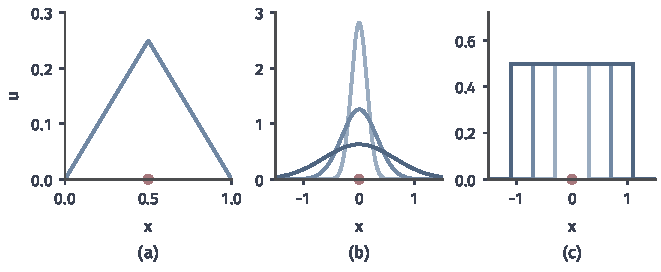
\includegraphics[width=112.0mm]{figures/06-differential-equations/02-partial-differential-equations/matplotlib/pdeprob-point-response/figure.pdf}
  \caption{对单位点刺激（红点）的响应。(a)$(0,1)$上的Poisson方程，解为折线。(b)实轴上的热方程，蓝色由浅到深为$t=0.01,0.05,0.2$，处处为正。(c)实轴上的波动方程，$c=1$，蓝色由浅到深为$t=0.3,0.7,1.1$，前沿之外为零。}
  \label{fig:pdeprob-point-response}
\end{BookInlineFigure}

表~\ref{tab:pdeprob-type-roles}汇总了这些差别，以及与之相配的数据。表中的结论是对模型方程而言的典型行为，一般方程要在相应条件下分别证明。

\begin{BookInlineTable}
  \centering
  \begin{tabular}{llll}
    \toprule
     & 椭圆型 & 抛物型 & 双曲型\\
    \midrule
    模型 & Poisson & 热 & 波动\\
    数据 & 全部边界 & 初值、侧面 & 两个初值、侧面\\
    传播 & 无时间方向 & 速度无穷 & 速度有限\\
    不光滑性 & 内部不产生 & 瞬间抹平 & 沿特征传播\\
    时间方向 & 无 & 不可逆 & 可逆\\
    \bottomrule
  \end{tabular}
  \caption{三类二阶模型方程的典型行为。}
  \label{tab:pdeprob-type-roles}
\end{BookInlineTable}

\paragraph{分类的适用范围}
类型是逐点定义的，系数随位置变化时类型可以改变。Tricomi方程$y\,\partial_x^{2}u+\partial_y^{2}u=0$的系数矩阵是$\operatorname{diag}(y,1)$：$y>0$时椭圆型，$y<0$时双曲型，$y=0$时退化。

在$y<0$的半平面，特征线满足$y\varphi_x^{2}+\varphi_y^{2}=0$，取$\varphi=x\mp\frac23(-y)^{3/2}$可以直接验证。图~\ref{fig:pdeprob-tricomi}中这两族曲线在下半平面交织，在$y=0$处形成尖点，上半平面没有特征线。这样的方程要在两个区域上分别提数据，不能套用单一类型的结论。

\begin{BookInlineFigure}
  \centering
  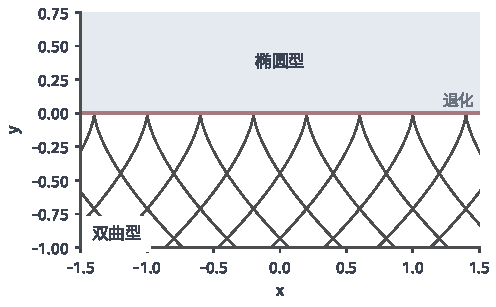
\includegraphics[width=84.0mm]{figures/06-differential-equations/02-partial-differential-equations/matplotlib/pdeprob-tricomi/figure.pdf}
  \caption{Tricomi方程$y\,\partial_x^2u+\partial_y^2u=0$的类型随位置变化。上半平面（浅蓝）椭圆型，红线$y=0$处退化，下半平面双曲型，深灰曲线是特征线$x\mp\frac23(-y)^{3/2}=$常数。}
  \label{fig:pdeprob-tricomi}
\end{BookInlineFigure}

分类也不记录变量的角色。方程$\partial_tu=\partial_x^{2}u$把$t$换成$-t$，得到$-\partial_tu=\partial_x^{2}u$，$\bm{M}$完全相同，仍是抛物型。但第一个方程向未来演化是好问题，向过去演化却不是，第~\ref{sec:pdeprob-well-posedness}节将具体算出差别。所以说一个方程是抛物型时，还要说明哪个变量是时间、沿哪个方向演化。

拟线性方程的主部系数依赖解，类型要在给定的解处判断，同一方程对不同的解可以不同。分类本身是线性方程的概念，推广到非线性方程总要先指明在哪个解上取线性化。

\paragraph{一阶方程按特征传播}
一阶方程没有二阶主部，二次型的分类对它们说不出什么，要改用另一种语言：信息沿曲线传递，这些曲线由常微分方程确定，同样称为特征线。

输运方程$\partial_tu+\bm{v}\cdot\nabla u=0$的特征线就是流体粒子的轨迹$\mathrm{d}\bm{x}/\mathrm{d}t=\bm{v}(\bm{x},t)$，它由给定的速度场决定，与解无关，沿线$u$不变。

非线性时情况改变。守恒律$\partial_tu+\partial_xF(u)=0$可以写成$\partial_tu+F'(u)\partial_xu=0$，信息的传播速度$F'(u)$依赖解本身，不同位置出发的曲线可能相交。Hamilton--Jacobi方程$\partial_tu+H(\nabla u)=0$对梯度非线性，沿曲线传递的是值和梯度，解在曲线相遇处会产生尖点。

这些方程的中心问题不是分类，而是相交之后如何选择解。这需要先搞清楚“解”究竟是什么意思。

\section{解的含义}
\label{sec:pdeprob-solutions}

到目前为止，“$u$满足方程”都是指把导数算出来、逐点代入。前面几个例子已经暴露了这种理解的局限：折线初值的折角在波动方程中一直存在，初值和边值不相容时输运方程的解带一条间断线。这些函数是不是解？要回答这个问题，就要明确“满足方程”的方式。

\paragraph{经典解}
最直接的要求是方程涉及的导数都存在且连续，方程逐点成立，初边值也逐点取到。

\begin{definition}[经典解]
\label{def:pdeprob-classical}
设$\Omega$是有界开集。Poisson方程$-\Delta u=f$配边值$u=g$的\term{经典解}（classical solution）是满足下列条件的函数：$u\in C^{2}(\Omega)\cap C(\overline{\Omega})$，在$\Omega$内每一点$-\Delta u=f$，在$\partial\Omega$上每一点$u=g$。对热方程问题~\eqref{eq:pdeprob-heat-ibvp}，经典解要求$u$对$\bm{x}$二阶、对$t$一阶连续可微于$\Omega\times(0,T]$，在$\overline{Q}$上连续，方程和初边值逐点成立。
\end{definition}

定义中的两层要求分工不同：内部的光滑性让方程有意义，到边界的连续性让边值有意义。热方程不要求光滑到$t=0$，正是为了容纳第~\ref{sec:pdeprob-initial}小节中的折线初值。

经典解的概念在两种情况下不够用：数据本身粗糙，或者解在演化中自己失去光滑性。下面逐一看。

\paragraph{粗糙的源项}
在$(0,1)$上考虑$-u''=f$，$u(0)=u(1)=0$，其中源项只在中间一段加热：
\begin{equation}
  f(x)=\begin{cases}4,&1/4<x<3/4,\\0,&\text{其他}.\end{cases}
  \label{eq:pdeprob-step-source}
\end{equation}
若$u\in C^{2}$，$u''$连续，但$u''=-f$在$x=1/4$处跳跃，所以经典解不存在。可是这根棒有确定的稳态温度，问题出在我们对“解”的要求太高。

分段把这个温度算出来。由对称性，$u'(1/2)=0$，所以在中段$u'(x)=-4(x-1/2)$，到左分界点时$u'(1/4)=1$。在$(0,1/4)$上$u''=0$，$u'$恒为$1$，由$u(0)=0$得
\[
  u(x)=x,\qquad 0\leq x\leq\frac14.
\]
中段积分一次得$u(x)=C-2(x-1/2)^{2}$，由$x=1/4$处连续，$C-\frac18=\frac14$，于是
\[
  u(x)=\frac38-2\Bigl(x-\frac12\Bigr)^{2},\qquad \frac14\leq x\leq\frac34.
\]
右段由对称性得$u(x)=1-x$。

这个函数在图~\ref{fig:pdeprob-weak-piecewise}中是一条光滑的曲线，$u$和$u'$都连续，只有$u''$在两个分界点跳跃。除这两点外方程逐点成立。我们希望有一种“解”的定义，能把它算进去，又不至于什么都算进去。

\begin{BookInlineFigure}
  \centering
  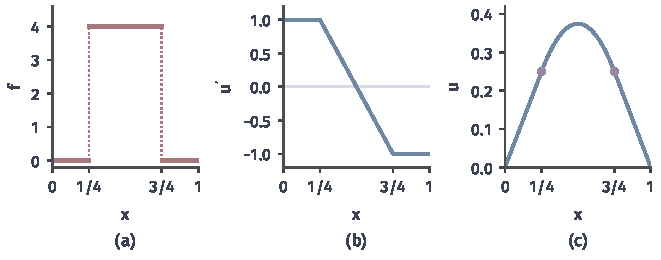
\includegraphics[width=112.0mm]{figures/06-differential-equations/02-partial-differential-equations/matplotlib/pdeprob-weak-piecewise/figure.pdf}
  \caption{跳跃源项下的解。(a)源项$f$，在$1/4$和$3/4$处跳跃。(b)$u'$连续，折点处$u''$跳跃。(c)$u$，紫点标出两个分界点，$u(1/2)=3/8$。}
  \label{fig:pdeprob-weak-piecewise}
\end{BookInlineFigure}

\paragraph{用测试函数检验}
把逐点检验换成加权平均的检验。逐点检验好比用一根无限细的探针逐点测量，而现实的探针总有一定宽度，读到的是附近的加权平均。两个函数相等，既可以逐点比较，也可以用所有光滑探针读数比较，后者不需要任何点上的导数。

设$\varphi$是\term{测试函数}（test function），即在$\Omega$内紧支撑的无穷次可微函数，全体记作$C_c^{\infty}(\Omega)$。若$u$是经典解，把$-\Delta u=f$乘以$\varphi$并在$\Omega$上积分，由分部积分得到
\[
  \int_\Omega\nabla u\cdot\nabla\varphi\,\mathrm{d}\bm{x}=\int_\Omega f\varphi\,\mathrm{d}\bm{x}.
\]
边界项因为$\varphi$在边界附近为零而消失。这个等式只含$u$的一阶导数，导数被挪了一阶到探针上。

把一阶导数也放宽，就要用到弱导数。设局部可积函数$w$对所有测试函数满足
\[
  \int_\Omega u\,\partial_{x_i}\varphi\,\mathrm{d}\bm{x}=-\int_\Omega w\,\varphi\,\mathrm{d}\bm{x},
\]
就称$w$是$u$的弱导数，这个$w$在几乎处处意义下唯一。详细的定义和性质可参考\BookChapterRef{chap:smoothing-weak-derivatives}{卷四第7章“光滑逼近与弱导数”}。

$H^{1}(\Omega)$由本身及各弱导数都属于$L^{2}(\Omega)$的函数组成，$H_0^{1}(\Omega)$是$C_c^{\infty}(\Omega)$在$H^{1}$范数下的闭包，在有界Lipschitz区域上恰好是边界迹为零的函数。这些空间的完备性、迹和嵌入性质可参考\BookChapterRef{chap:sobolev-spaces}{卷四第21章“Sobolev空间”}。

\begin{definition}[Poisson方程的弱解]
\label{def:pdeprob-weak-poisson}
设$\Omega\subset\mathbb{R}^{d}$是有界开集，$f\in L^{2}(\Omega)$。若$u\in H_0^{1}(\Omega)$满足
\begin{equation}
  \begin{gathered}
    a(u,v)=\int_\Omega fv\,\mathrm{d}\bm{x},\qquad\forall v\in H_0^{1}(\Omega),\\
    a(u,v)=\int_\Omega\nabla u\cdot\nabla v\,\mathrm{d}\bm{x},
  \end{gathered}
  \label{eq:pdeprob-weak-form}
\end{equation}
则称$u$是零边值Poisson问题的\term{弱解}（weak solution），式~\eqref{eq:pdeprob-weak-form}称为它的\term{弱形式}（weak formulation）。
\end{definition}

定义的三个成分各有作用。要求$u\in H^{1}$，式~\eqref{eq:pdeprob-weak-form}左边才有意义；要求$u\in H_0^{1}$，把零边值写进了解所在的空间；让$v$取遍$H_0^{1}$而非只取测试函数，并没有增加要求，因为测试函数在其中稠密、等式两边对$v$连续。

分段例子的$u$是弱解。$u$连续可微且在两端为零，所以$u\in H_0^{1}(0,1)$。对测试函数$\varphi$，把积分分成三段分别分部积分：
\[
  \int_0^{1}u'\varphi'\,\mathrm{d}x
  =\sum_{\text{三段}}\Bigl(\bigl[u'\varphi\bigr]-\int u''\varphi\,\mathrm{d}x\Bigr).
\]
$u'$在两个分界点连续，相邻两段的端点项互相抵消，$\varphi$在$0,1$处为零，端点项全部消失。各段内$-u''=f$，于是
\[
  \int_0^{1}u'\varphi'\,\mathrm{d}x=\int_0^{1}f\varphi\,\mathrm{d}x.
\]

弱解的要求并不是“几乎处处满足方程”。在$(0,1)$上取$f=0$，考虑折线$u=\min\{x,1-x\}$，除$x=1/2$外$u''=0$，两端也为零。它是不是$-u''=0$的弱解？取测试函数$\varphi$，同样分段，$u'$在$(0,1/2)$上是$1$，在$(1/2,1)$上是$-1$：
\[
  \int_0^{1}u'\varphi'\,\mathrm{d}x
  =\int_0^{1/2}\varphi'\,\mathrm{d}x-\int_{1/2}^{1}\varphi'\,\mathrm{d}x
  =2\varphi\Bigl(\frac12\Bigr).
\]

结果不为零，所以折线不是弱解：探针读出了折点。这个折点实际上是一个集中在$x=1/2$、强度为$2$的点热源，第~\ref{sec:pdeprob-types}节的点源解就是这一函数的一半。

图~\ref{fig:pdeprob-kink-test}取一个具体的光滑探针演示，(b)中$u'\varphi'$在两侧都是正的，面积加起来等于$2\varphi(1/2)=2$。“几乎处处”忽略了一点上发生的事，而测试函数不会。

\begin{BookInlineFigure}
  \centering
  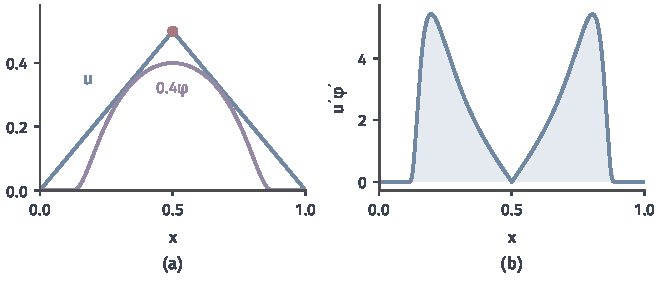
\includegraphics[width=112.0mm]{figures/06-differential-equations/02-partial-differential-equations/matplotlib/pdeprob-kink-test/figure.pdf}
  \caption{探针读出折点。(a)折线$u=\min\{x,1-x\}$（蓝，红点为折点）与测试函数$\varphi(x)=\exp(1-1/(1-r^2))$，$r=(x-\frac12)/0.4$（紫，图中缩放$0.4$倍）。(b)$u'\varphi'$，阴影面积的数值积分为$2.000$，等于$2\varphi(\frac12)$。}
  \label{fig:pdeprob-kink-test}
\end{BookInlineFigure}

弱解是经典解的推广，而不是另一种东西。下面的定理说明，函数足够光滑时两者一致。

\begin{theorem}[弱解与经典解的相容]
\label{thm:pdeprob-weak-classical}
设$\Omega$是有界Lipschitz区域，$f\in C(\overline{\Omega})$，$u\in C^{2}(\overline{\Omega})$且在$\partial\Omega$上$u=0$。则$u$是经典解，当且仅当$u$满足弱形式~\eqref{eq:pdeprob-weak-form}。
\end{theorem}

\begin{proof}
$u$连续可微到边界且边界值为零，所以$u\in H_0^{1}(\Omega)$。对$v\in C_c^{\infty}(\Omega)$，由乘积法则，
\[
  \nabla\cdot(v\nabla u)=\nabla v\cdot\nabla u+v\Delta u.
\]
$v$在边界附近为零，由散度定理，左边的积分为零，于是
\[
  \int_\Omega\nabla u\cdot\nabla v\,\mathrm{d}\bm{x}=-\int_\Omega v\,\Delta u\,\mathrm{d}\bm{x}.
\]

若$u$是经典解，右边等于$\int_\Omega fv\,\mathrm{d}\bm{x}$，对测试函数成立。式~\eqref{eq:pdeprob-weak-form}两边都是$v$在$H^{1}$范数下的连续线性泛函，由稠密性，等式对全部$v\in H_0^{1}(\Omega)$成立。

反过来，若弱形式成立，则对任意测试函数$v$有
\[
  \int_\Omega(-\Delta u-f)\,v\,\mathrm{d}\bm{x}=0.
\]
$-\Delta u-f$连续。若它在某点为正，取在该点附近非负、不恒为零的测试函数$v$，积分为正，矛盾；为负时同理。所以$-\Delta u=f$在$\Omega$内处处成立。
\end{proof}

\paragraph{演化产生的间断}
第二种情况更棘手：数据没有间断，解却在有限时间内失去光滑性。考虑守恒律$\partial_tu+\partial_x(u^{2}/2)=0$，即拟线性方程$\partial_tu+u\,\partial_xu=0$，通常称为Burgers方程。沿直线$x=x_0+u_0(x_0)t$，
\[
  \frac{\mathrm{d}}{\mathrm{d}t}u(x_0+u_0(x_0)t,t)=\partial_tu+u_0(x_0)\partial_xu=0.
\]
所以$u$沿这条直线保持初值$u_0(x_0)$，初值大的点跑得快。

取初值
\begin{equation}
  u_0(x)=\begin{cases}1,&x<0,\\1-x,&0\leq x\leq1,\\0,&x>1.\end{cases}
  \label{eq:pdeprob-burgers-ramp}
\end{equation}
由$x=x_0+(1-x_0)t$解出$x_0=(x-t)/(1-t)$，在$t<1$时得到
\[
  u(x,t)=\frac{1-x}{1-t},\qquad t\leq x\leq1.
\]
这时$\partial_xu=-1/(1-t)$，$t\to1$时斜率趋于无穷。图~\ref{fig:pdeprob-burgers-crossing}(a)中，从$[0,1]$出发的直线全部在$(1,1)$汇聚；(b)中坡面越来越陡，$t=1$时成为垂直的台阶。此后沿直线算出的值成为多值，方程必须换一种读法。斜坡的两个折角只是为了算得出显式解，把它磨成无穷次可微的初值，坡面同样会在有限时间变成垂直。

\begin{BookInlineFigure}
  \centering
  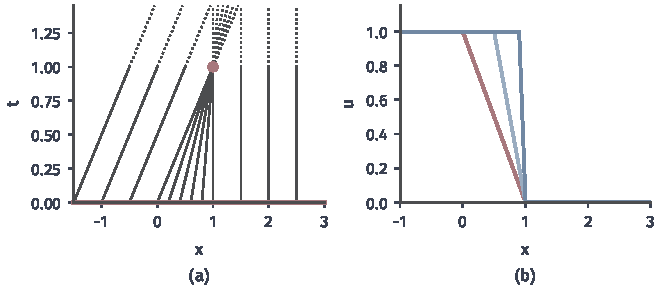
\includegraphics[width=112.0mm]{figures/06-differential-equations/02-partial-differential-equations/matplotlib/pdeprob-burgers-crossing/figure.pdf}
  \caption{Burgers方程的斜坡初值。(a)从初始线（红）出发的直线$x=x_0+u_0(x_0)t$（深灰），在红点$(1,1)$汇聚，虚线部分表示相交后已无法继续沿用。(b)解的形状，红线为$t=0$，蓝色由浅到深为$t=0.5,0.9$。}
  \label{fig:pdeprob-burgers-crossing}
\end{BookInlineFigure}

同样的办法可以用在这里，但必须从守恒形式出发。设$u$是光滑解，把$\partial_tu+\partial_xF(u)=0$乘以$\varphi\in C_c^{\infty}(\mathbb{R}\times[0,\infty))$，在$\mathbb{R}\times(0,\infty)$上积分并分部积分，所有导数都转到$\varphi$上：
\begin{equation}
  \int_0^{\infty}\!\!\int_{\mathbb{R}}\bigl(u\,\partial_t\varphi+F(u)\,\partial_x\varphi\bigr)\,\mathrm{d}x\,\mathrm{d}t
  +\int_{\mathbb{R}}u_0\,\varphi(\cdot,0)\,\mathrm{d}x=0.
  \label{eq:pdeprob-weak-conservation}
\end{equation}
$\varphi$在$t=0$可以不为零，第二项由此而来，初值由它写进方程。局部有界可测函数$u$若对所有这样的$\varphi$满足式~\eqref{eq:pdeprob-weak-conservation}，就称为守恒律的弱解。这个式子里没有$u$的导数，间断的$u$也可以代入。

必须强调从守恒形式出发。$u\,\partial_xu$在$u$间断时没有定义，而$\partial_x(u^{2}/2)$可以用弱导数理解。两种写法对光滑解等价，对间断解不等价。

线性方程的粗糙解也用同样的方式理解。输运方程带间断线的解~\eqref{eq:pdeprob-transport-solution}和波动方程带折角的解，都可以看成光滑解的极限；把导数全部转到测试函数上之后，积分等式在极限下保持成立，它们因此是弱解。这回答了本节开头的问题。

\paragraph{弱解可以不唯一}
放宽到这一步后，又出现了新问题。下面算出间断解需要满足的条件。设$u$在直线$x=st$左侧为常数$u_l$，右侧为常数$u_r$，初值是相应的台阶。在左侧区域上对向量场$(F(u_l)\varphi,u_l\varphi)$用散度定理，这个区域的边界由$t=0$的半直线和$x=st$组成，得到
\[
  \begin{aligned}
  &\iint_{x<st}\bigl(u_l\partial_t\varphi+F(u_l)\partial_x\varphi\bigr)\,\mathrm{d}x\,\mathrm{d}t\\
  &\qquad=\int_0^{\infty}\bigl(F(u_l)-su_l\bigr)\varphi(st,t)\,\mathrm{d}t
  -\int_{-\infty}^{0}u_l\varphi(x,0)\,\mathrm{d}x.
  \end{aligned}
\]
右侧区域的计算相同，只是直线上的外法向反号。两式相加，再加上式~\eqref{eq:pdeprob-weak-conservation}的初值项，初值积分全部抵消，只剩直线上的积分：
\[
  \int_0^{\infty}\bigl(F(u_l)-F(u_r)-s(u_l-u_r)\bigr)\varphi(st,t)\,\mathrm{d}t=0.
\]
对所有$\varphi$成立，当且仅当间断速度满足
\begin{equation}
  s\,(u_r-u_l)=F(u_r)-F(u_l).
  \label{eq:pdeprob-jump-condition}
\end{equation}

现在取Burgers方程，$F(u)=u^{2}/2$，初值在$x<0$时为$0$，$x>0$时为$1$。下面两个函数都是弱解。第一个是间断解：$u_l=0$，$u_r=1$，由式~\eqref{eq:pdeprob-jump-condition}，$s=\frac12$，
\[
  u^{\mathrm{a}}(x,t)=\begin{cases}0,&x<t/2,\\1,&x>t/2.\end{cases}
\]
第二个是连续的扇形：
\[
  u^{\mathrm{b}}(x,t)=\begin{cases}0,&x\leq0,\\x/t,&0<x<t,\\1,&x\geq t.\end{cases}
\]
扇形内部$\partial_tu+u\,\partial_xu=-x/t^{2}+(x/t)(1/t)=0$，它在两条分界线上连续，分段积分时端点项抵消，所以也满足式~\eqref{eq:pdeprob-weak-conservation}。

一个初值对应两个弱解，弱形式提供的信息不足以挑出一个。图~\ref{fig:pdeprob-riemann}(a)中，$u^{\mathrm{a}}$两侧的特征线都从间断处发出，好比信息从间断线上凭空产生，这在物理上不合理；(b)中的$u^{\mathrm{b}}$没有这个问题。(c)给方程加上一个很小的黏性项，算出来的解贴近$u^{\mathrm{b}}$。

\begin{BookInlineFigure}
  \centering
  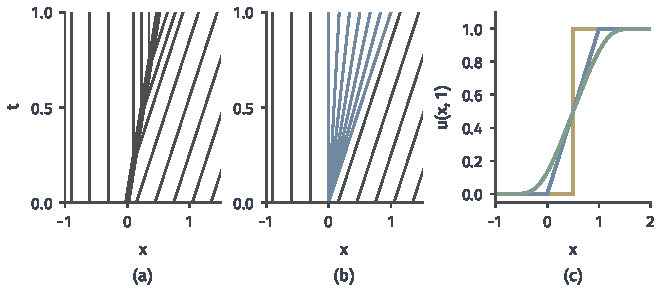
\includegraphics[width=112.0mm]{figures/06-differential-equations/02-partial-differential-equations/matplotlib/pdeprob-riemann/figure.pdf}
  \caption{同一台阶初值的两个弱解。(a)间断解：深灰粗线是间断线$x=t/2$，细线是特征线，它们都从间断线离开。(b)扇形解：蓝线是从原点发出的扇形特征线。(c)$t=1$的形状：间断解（黄）、扇形解（蓝）、带黏性$\nu=0.02$的数值解（绿）。}
  \label{fig:pdeprob-riemann}
\end{BookInlineFigure}

要恢复唯一性，就要在弱解中增加一条选择规则，只保留与小黏性极限一致的解。满足这种规则的弱解称为\term{熵解}（entropy solution），第~\ref{chap:scalar-conservation-laws}章给出精确的定义并证明唯一性。

\paragraph{Hamilton--Jacobi方程：几乎处处太宽}
最后一种情况说明，弱导数的办法并不总能用上。考虑$\lvert u'\rvert=1$，$x\in(-1,1)$，$u(\pm1)=0$，这是从边界出发、速度为$1$的波前的到达时间所满足的方程。

它没有$C^{1}$解。若$u\in C^{1}$，由Rolle定理存在一点$u'=0$，与$\lvert u'\rvert=1$矛盾。若只要求几乎处处成立，又有太多的解：图~\ref{fig:pdeprob-eikonal}(a)中每一条锯齿线的斜率都是$\pm1$，可以折任意多次。

这里不能把导数转到测试函数上，因为方程对$u'$非线性，$\lvert u'\rvert$无法通过分部积分移走。可行的选择办法仍然是加小黏性。考虑
\[
  (u')^{2}-\varepsilon u''=1,\qquad u(\pm1)=0.
\]
它有显式解
\begin{equation}
  u_\varepsilon(x)=\varepsilon\Bigl(\ln\cosh\frac{1}{\varepsilon}-\ln\cosh\frac{x}{\varepsilon}\Bigr).
  \label{eq:pdeprob-viscous-eikonal}
\end{equation}

下面验证。两次求导得到
\[
  u_\varepsilon'=-\tanh\frac{x}{\varepsilon},\qquad
  u_\varepsilon''=-\frac{1}{\varepsilon}\operatorname{sech}^{2}\frac{x}{\varepsilon}.
\]
于是
\[
  (u_\varepsilon')^{2}-\varepsilon u_\varepsilon''=\tanh^{2}\frac{x}{\varepsilon}+\operatorname{sech}^{2}\frac{x}{\varepsilon}=1.
\]
边值也满足，因为$\cosh$是偶函数。令$\varepsilon\to0$，由$\cosh s\approx\frac12\mathrm{e}^{\lvert s\rvert}$（$\lvert s\rvert$很大时），
\[
  \varepsilon\ln\cosh\frac{x}{\varepsilon}\to\lvert x\rvert,
\]
所以$u_\varepsilon\to1-\lvert x\rvert$。这正是到边界的距离，即波前的最短到达时间。图~\ref{fig:pdeprob-eikonal}(b)显示了这个极限。

\begin{BookInlineFigure}
  \centering
  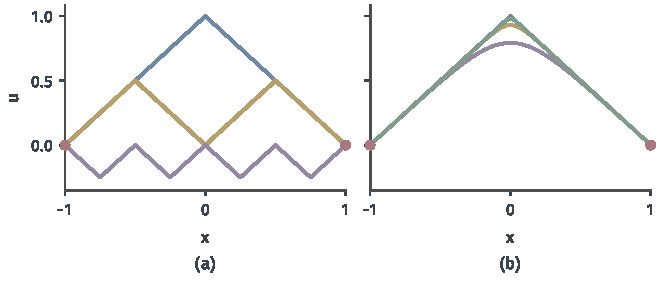
\includegraphics[width=112.0mm]{figures/06-differential-equations/02-partial-differential-equations/matplotlib/pdeprob-eikonal/figure.pdf}
  \caption{$\lvert u'\rvert=1$，$u(\pm1)=0$（红点）。(a)几个几乎处处满足方程的函数：$1-\lvert x\rvert$（蓝）和两条锯齿线（黄、紫）。(b)小黏性解$u_\varepsilon$，$\varepsilon=0.3$（紫）、$0.1$（黄）、$0.03$（绿）趋于$1-\lvert x\rvert$（蓝）。}
  \label{fig:pdeprob-eikonal}
\end{BookInlineFigure}

注意$\varepsilon$前的符号决定了选中的解：把$-\varepsilon u''$换成$+\varepsilon u''$，极限就成了$\lvert x\rvert-1$。这条选择规则的严格形式不用导数，而是在解被光滑函数从上方或下方触碰的点上提出不等式，满足它的解称为\term{黏性解}（viscosity solution），第~\ref{chap:hamilton-jacobi-equations}章专门讨论。

表~\ref{tab:pdeprob-solution-concepts}对比了这几种解的概念。它们不是彼此竞争的定义，而是针对不同方程结构的不同检验方式，光滑时都回到经典解。

\begin{BookInlineTable}
  \centering
  \begin{tabular}{lll}
    \toprule
    解的概念 & 检验方式 & 用在哪里\\
    \midrule
    经典解 & 逐点代入导数 & 数据和解都足够光滑\\
    弱解 & 导数转到测试函数上 & 方程有散度结构\\
    熵解 & 弱解，加熵条件 & 标量守恒律\\
    黏性解 & 用光滑函数从两侧触碰 & Hamilton--Jacobi方程\\
    \bottomrule
  \end{tabular}
  \caption{几种解的概念。}
  \label{tab:pdeprob-solution-concepts}
\end{BookInlineTable}

\section{适定性}
\label{sec:pdeprob-well-posedness}

写出一个公式，是否就解决了问题？细棒的热方程反向求解也有“公式”：把初值的正弦系数乘上一个增长的指数，形式上和正向完全对称。下面会看到，这个公式几乎没有用处。判断一个问题是否提得合理，需要把三个问题分开回答。

\paragraph{三个问题}
把问题看成从数据到解的一个映射。这个映射要有意义，至少要回答：对给定的数据，解存在吗？解只有一个吗？数据有小的误差时，解的变化也小吗？这三个问题只有在明确了数据和解分别属于什么空间、用什么范数度量之后，才有确切的答案。

\begin{definition}[适定问题]
\label{def:pdeprob-well-posed}
设数据空间$D$和解空间$S$是赋范空间。若对每个$d\in D$，问题在$S$中存在唯一的解$\mathcal{S}(d)$，且映射$\mathcal{S}:D\to S$连续，即
\begin{equation}
  \lVert d_n-d\rVert_{D}\to0\ \Longrightarrow\ \lVert\mathcal{S}(d_n)-\mathcal{S}(d)\rVert_{S}\to0,
  \label{eq:pdeprob-continuous-dependence}
\end{equation}
就称问题在$(D,S)$下是\term{适定问题}（well-posed problem），否则称为\term{不适定问题}（ill-posed problem）。
\end{definition}

这是Hadamard提出的标准。线性问题中$\mathcal{S}$是线性映射，连续性等价于存在常数$C$，使得
\[
  \lVert\mathcal{S}(d)\rVert_{S}\leq C\lVert d\rVert_{D},\qquad\forall d\in D.
\]

图~\ref{fig:pdeprob-well-posed-map}画出了这三条要求：每个数据都有箭头指出（存在），箭头只有一支（唯一），数据的邻域映到解的小邻域（连续依赖）。线性算子方程的相应结论，可参考\BookChapterRef{chap:linear-operator-equations}{卷四第19章“线性算子方程”}。

\begin{BookInlineFigure}
  \centering
  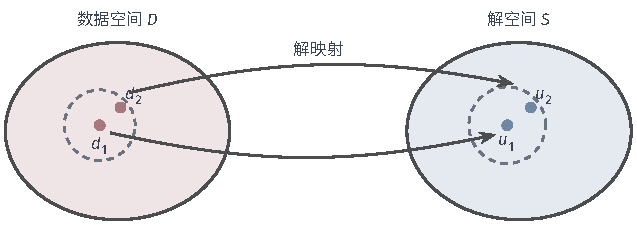
\includegraphics[width=107.8mm]{figures/06-differential-equations/02-partial-differential-equations/tikz/pdeprob-well-posed-map/figure.pdf}
  \caption{适定性是从数据空间到解空间的连续映射。虚线圈分别表示所选范数下的邻域，相近的数据$d_1,d_2$对应相近的解$u_1,u_2$。换一对空间，三条要求的答案都可能改变。}
  \label{fig:pdeprob-well-posed-map}
\end{BookInlineFigure}

\paragraph{存在：解空间是否够大}
存在性的答案依赖解空间。跳跃源项~\eqref{eq:pdeprob-step-source}在$C^{2}$中没有解，在$H_0^{1}$中有解；Neumann问题在数据违反式~\eqref{eq:pdeprob-neumann-compat}时哪里都没有解，这时要把数据空间缩小到满足约束的子空间。

非线性方程的存在性还有时间范围的问题。对Burgers方程，沿直线$x=x_0+u_0(x_0)t$，对$x_0$求导可得
\[
  \partial_xu=\frac{u_0'(x_0)}{1+u_0'(x_0)\,t}.
\]
只要某处$u_0'<0$，分母就会在有限时间变为零，光滑解只能存在到
\begin{equation}
  T^{*}=-\frac{1}{\min_xu_0'(x)}.
  \label{eq:pdeprob-burgers-breaking}
\end{equation}
式~\eqref{eq:pdeprob-burgers-ramp}的斜坡初值中$\min u_0'=-1$，$T^{*}=1$，与图~\ref{fig:pdeprob-burgers-crossing}一致。在$C^{1}$中只有局部解，放宽到弱解后解可以延续到所有时间。这和第~\ref{chap:ode-existence-continuation}章的情形类似，那里常微分方程的解也可能在有限时间爆炸，不过这里爆炸的是导数，而解本身仍然有界。

\paragraph{唯一：解空间是否够小}
解空间放得太大，唯一性就会失去，上一节的两个弱解和无穷多条锯齿线都是例子。Neumann问题差一个常数，这时要在解空间上加均值为零的条件，或者把差常数的函数视为同一个。

对线性演化方程，证明唯一性最常用的工具是能量估计：对两个解的差构造一个非负量，证明它不增。下面的定理同时给出唯一性和连续依赖。

\begin{theorem}[细棒热方程的能量估计]
\label{thm:pdeprob-heat-energy}
设$u_1,u_2$在$[0,1]\times[0,T]$上连续，$\partial_tu_i$、$\partial_xu_i$、$\partial_x^{2}u_i$在同一闭集上连续，满足同一方程$\partial_tu=\partial_x^{2}u+f$和同一边值$u(0,t)=g_0(t)$、$u(1,t)=g_1(t)$。则对$t\in[0,T]$，
\begin{equation}
  \lVert u_1(\cdot,t)-u_2(\cdot,t)\rVert_{L^{2}(0,1)}\leq\lVert u_1(\cdot,0)-u_2(\cdot,0)\rVert_{L^{2}(0,1)}.
  \label{eq:pdeprob-heat-energy}
\end{equation}
特别地，初值相同的两个解相等。
\end{theorem}

\begin{proof}
记$w=u_1-u_2$。由线性，$w$满足$\partial_tw=\partial_x^{2}w$，两端值为零。定义
\[
  E(t)=\frac12\int_0^{1}w(x,t)^{2}\,\mathrm{d}x.
\]
$\partial_tw$在闭集上连续，可以在积分号下求导，再代入方程：
\[
  E'(t)=\int_0^{1}w\,\partial_tw\,\mathrm{d}x=\int_0^{1}w\,\partial_x^{2}w\,\mathrm{d}x.
\]
分部积分，端点项$[w\,\partial_xw]_0^{1}$因$w$在两端为零而消失：
\[
  E'(t)=-\int_0^{1}(\partial_xw)^{2}\,\mathrm{d}x\leq0.
\]
所以$E(t)\leq E(0)$，开方即得式~\eqref{eq:pdeprob-heat-energy}。初值相同时$E(0)=0$，于是$E\equiv0$，$w\equiv0$。
\end{proof}

定理中的条件要求解光滑到初始时刻和边界。在无界区域上，单凭方程和初值并不能保证唯一性：实轴上的热方程存在初值为零、但不恒为零的解，它们在$\lvert x\rvert\to\infty$时增长得极快。这个构造由Tikhonov给出，证明需要较长的级数估计，读者可查阅偏微分方程教材。加上增长限制$\lvert u(x,t)\rvert\leq C\mathrm{e}^{ax^{2}}$后唯一性恢复，这说明解空间的限制不是技术细节。

\paragraph{连续依赖：同一方程，两个方向}
现在回到本节开头的问题。设$u_0=\sum_kb_k\sin k\pi x$，$u$是细棒两端为零的热方程的解，则第$k$个模式的系数在时刻$t$变为$b_k\mathrm{e}^{-k^{2}\pi^{2}t}$。由正弦函数的正交性，$\lVert\sin k\pi x\rVert_{L^{2}(0,1)}^{2}=\frac12$，于是
\[
  \lVert u(\cdot,T)\rVert_{L^{2}(0,1)}^{2}
  =\frac12\sum_kb_k^{2}\mathrm{e}^{-2k^{2}\pi^{2}T}
  \leq\lVert u_0\rVert_{L^{2}(0,1)}^{2}.
\]
正向映射$u_0\mapsto u(\cdot,T)$在$L^{2}$上有界，高频模式被强烈衰减。

反过来，由$T$时刻的温度$d=\sum_kd_k\sin k\pi x$推算初始温度，公式也可以写出来：
\begin{equation}
  u(x,0)=\sum_{k\geq1}d_k\,\mathrm{e}^{k^{2}\pi^{2}T}\sin k\pi x.
  \label{eq:pdeprob-backward-heat}
\end{equation}
形式上它和正向一样简单，但指数的符号反了。图~\ref{fig:pdeprob-backward-heat}(a)比较了两个方向上各模式的放大倍数。

这个公式首先不保证解存在。要让式~\eqref{eq:pdeprob-backward-heat}属于$L^{2}$，$d_k$必须满足$\sum_kd_k^{2}\mathrm{e}^{2k^{2}\pi^{2}T}<\infty$。折线$\min\{x,1-x\}$的系数只有$k^{-2}$的量级，不满足这个条件，它不可能是任何$L^{2}$初值在正时刻的温度。这和正向热方程瞬间变光滑是同一件事。

唯一性倒还成立：若$d=0$，每个$d_k$为零，$L^{2}$初值的所有系数都为零。问题出在连续依赖。取数据的扰动$\delta=\varepsilon\sin k\pi x$，它的$L^{2}$范数是$\varepsilon/\sqrt{2}$，反算出的初值扰动是
\[
  \varepsilon\,\mathrm{e}^{k^{2}\pi^{2}T}\sin k\pi x,
\]
放大倍数是$\mathrm{e}^{k^{2}\pi^{2}T}$，随$k$无界增长。所以反向映射在$L^{2}$上无界，问题在$(L^{2},L^{2})$下不适定。

下面取具体的数字。$T=0.1$，真实初值$\sin\pi x$，它在$T$时刻的温度是$\mathrm{e}^{-\pi^{2}T}\sin\pi x$。给这个数据加上幅度$\varepsilon=10^{-10}$的第$5$模式扰动，反算时模式$5$的放大倍数是
\[
  \mathrm{e}^{25\pi^{2}\cdot0.1}\approx5.2\times10^{10},
\]
反算结果中出现幅度约$5.2$的振荡。图~\ref{fig:pdeprob-backward-heat}(b)中，真实解的幅度为$1$，几乎完全被这个振荡淹没，而数据的扰动只有$10^{-10}$，小于任何测量误差。

\begin{BookInlineFigure}
  \centering
  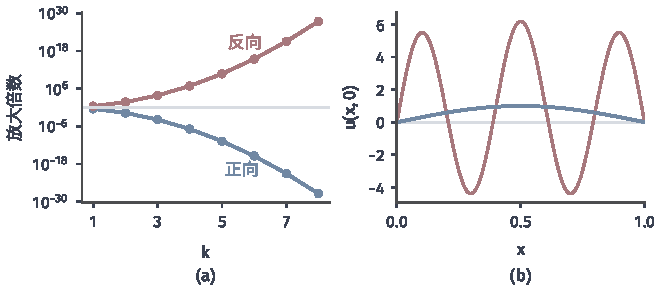
\includegraphics[width=112.0mm]{figures/06-differential-equations/02-partial-differential-equations/matplotlib/pdeprob-backward-heat/figure.pdf}
  \caption{热方程的两个方向，$T=0.1$。(a)第$k$个模式的放大倍数：正向$\mathrm{e}^{-k^2\pi^2T}$（蓝）与反向$\mathrm{e}^{k^2\pi^2T}$（红），纵轴为对数坐标。(b)真实初值$\sin\pi x$（蓝）与数据含幅度$10^{-10}$的第$5$模式扰动时的反算结果（红）。}
  \label{fig:pdeprob-backward-heat}
\end{BookInlineFigure}

适定性是相对于空间而言的，这里可以看得很清楚。若把数据空间的范数改为
\[
  \lVert d\rVert_{*}^{2}=\frac12\sum_kd_k^{2}\mathrm{e}^{2k^{2}\pi^{2}T},
\]
反向映射就成了等距映射，问题“适定”了。但这个范数下的小，意味着高频分量小到指数级，现实的测量误差达不到，这种适定性没有实用价值。选择空间时要问：数据的误差实际上在什么范数下小？

\paragraph{同一方程，换一种数据}
椭圆方程有一个著名的类似例子，说明同一方程配不同的数据，结果可以完全不同。考虑上半平面上的Laplace方程，把$y$当作“时间”，像波动方程那样给两个初值：
\begin{equation}
  \partial_x^{2}u+\partial_y^{2}u=0,\qquad
  u(x,0)=0,\qquad \partial_yu(x,0)=\frac{\sin kx}{k}.
  \label{eq:pdeprob-hadamard}
\end{equation}
直接代入可以验证，解是
\[
  u(x,y)=\frac{\sinh(ky)\sin kx}{k^{2}}.
\]

$k\to\infty$时，数据一致地趋于零，解却对每个$y>0$都按$\mathrm{e}^{ky}/(2k^{2})$爆炸。$k=20$时，数据的幅度只有$0.05$，在$y=1$处解的幅度是$\sinh(20)/400\approx6.1\times10^{5}$。图~\ref{fig:pdeprob-hadamard}画出了这种增长。若把数据换成$\sin(kx)/k^{m}$，数据的任意有限阶导数都趋于零，指数增长依然如故。

\begin{BookInlineFigure}
  \centering
  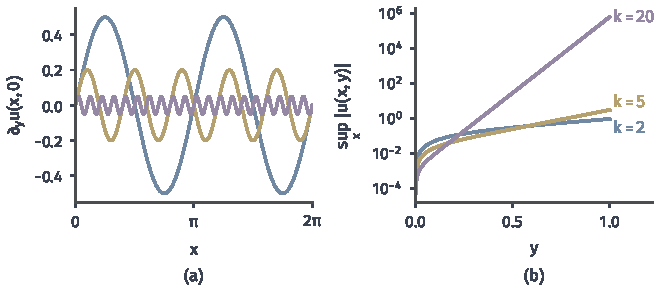
\includegraphics[width=112.0mm]{figures/06-differential-equations/02-partial-differential-equations/matplotlib/pdeprob-hadamard/figure.pdf}
  \caption{Laplace方程的“初值”问题~\eqref{eq:pdeprob-hadamard}。(a)数据$\partial_yu(x,0)=\sin(kx)/k$，$k=2$（蓝）、$5$（黄）、$20$（紫），频率越高幅度越小。(b)解的幅度$\sinh(ky)/k^2$随$y$的增长，纵轴为对数坐标。频率最高的数据最小，增长最快。}
  \label{fig:pdeprob-hadamard}
\end{BookInlineFigure}

同一方程配Dirichlet数据却是适定的。在$(0,1)$上取$-u''=f$，$u(0)=u(1)=0$，先对解本身做能量估计。将方程乘以$u$并分部积分，端点项消失：
\[
  \lVert u'\rVert_{L^{2}}^{2}=\int_0^{1}fu\,\mathrm{d}x\leq\lVert f\rVert_{L^{2}}\lVert u\rVert_{L^{2}}.
\]
再把$u$展开成正弦级数$\sum_kc_k\sin k\pi x$，由$k\geq1$，
\[
  \lVert u'\rVert_{L^{2}}^{2}=\frac12\sum_kk^{2}\pi^{2}c_k^{2}\geq\pi^{2}\lVert u\rVert_{L^{2}}^{2},
\]
这是区间上的Poincaré不等式。把它代入上式右端，两边约去$\lVert u'\rVert_{L^{2}}$，得到
\begin{equation}
  \lVert u'\rVert_{L^{2}(0,1)}\leq\frac{1}{\pi}\lVert f\rVert_{L^{2}(0,1)}.
  \label{eq:pdeprob-poisson-energy}
\end{equation}
取$u=\sin\pi x$，$f=\pi^{2}\sin\pi x$时，两边都是$\pi/\sqrt{2}$，等号成立。由线性，这个估计同时给出唯一性和对$f$的连续依赖，存在性由第~\ref{chap:elliptic-equations}章的变分方法给出。

波动方程的估计量不同。设$u$在$[0,1]\times[0,T]$上二阶连续可微，满足$\partial_t^{2}u=c^{2}\partial_x^{2}u$和零边值，定义能量
\[
  E(t)=\frac12\int_0^{1}\bigl((\partial_tu)^{2}+c^{2}(\partial_xu)^{2}\bigr)\,\mathrm{d}x.
\]
求导并对第二项分部积分，端点上$\partial_tu=0$，于是
\begin{equation}
  E'(t)=\int_0^{1}\partial_tu\,\bigl(\partial_t^{2}u-c^{2}\partial_x^{2}u\bigr)\,\mathrm{d}x=0.
  \label{eq:pdeprob-wave-energy}
\end{equation}
能量守恒，对时间的两个方向都成立，这正是波动方程可逆的反映。它要求数据是一对函数，数据空间自然取$H_0^{1}(0,1)\times L^{2}(0,1)$，而不是$L^{2}$。

\paragraph{不同数据要求下的结果}
表~\ref{tab:pdeprob-well-posed-summary}把本章的例子放在一起。前两行方程相同、方向相反，第三、四行方程相同、数据位置不同，每一行都要连同空间一起读。其中Laplace方程Cauchy问题的唯一性来自调和函数的解析性，Burgers方程熵解的结论在第~\ref{chap:scalar-conservation-laws}章讨论，这里只记录结果。

\begin{BookInlineTable}
  \centering
  \begin{tabular}{llll}
    \toprule
    问题与空间 & 存在 & 唯一 & 连续依赖\\
    \midrule
    热方程正向，$L^{2}$ & 有 & 有 & 有\\
    热方程反向，$L^{2}$ & 一般无 & 有 & 无\\
    Poisson，Dirichlet，$H_0^{1}$ & 有 & 有 & 有\\
    Laplace，Cauchy数据 & 一般无 & 有 & 无\\
    Poisson，Neumann & 需式~\eqref{eq:pdeprob-neumann-compat} & 差常数 & 商掉常数后有\\
    Burgers，$C^{1}$ & 仅到$T^{*}$ & 有 & 局部有\\
    Burgers，弱解 & 有 & 无 & 无从谈起\\
    Burgers，熵解 & 有 & 有 & 有\\
    \bottomrule
  \end{tabular}
  \caption{同一方程在不同数据与空间要求下的适定性。}
  \label{tab:pdeprob-well-posed-summary}
\end{BookInlineTable}

适定也不等于计算容易。连续依赖只说误差放大倍数有限，这个倍数可能很大；离散后的方程是否继承连续问题的稳定性，是另一个问题，要在第~\ref{chap:pde-numerical-methods}章对具体格式讨论。

\section{本章小结}
\label{sec:pdeprob-summary}

一个偏微分方程问题由四样东西共同构成：未知场和它所在的区域，方程本身，初值和边界数据，以及“解”的含义和相应的函数空间。只写一条方程不等于提出了问题，$\partial_tu=\partial_x^{2}u$有无穷多解，它们的差别要由数据来确定。

未知量从向量变成函数后，方程可以由局部守恒和具体的通量规律得出，Poisson、输运、热和波动四个模型都写成同一组变量。空间离散后，热方程就是常微分方程组，但矩阵的谱范数按$4/h^{2}$增长，所以不能把常微分方程的存在性定理直接搬过来。

需要什么数据由方程决定。时间阶数决定初始函数的个数，边界条件可以规定场值、通量或两者的组合，输运方程只在入流边界给数据。初值与边值在角点要相容，相容的阶数随所要求的光滑性增加；Neumann问题还有积分约束。不是数据越多越好。

对二阶线性方程，系数矩阵特征值的符号结构决定类型：椭圆型受整个边界约束，抛物型立刻抹平，双曲型以有限速度传播不光滑性。类型在坐标变换下不变，但是逐点定义，也不记录时间的方向。一阶方程不在这个分类中，它们按特征线传播，非线性时特征线会相交。

数据粗糙或演化产生间断时，要改变方程成立的方式。弱解把导数转移到测试函数上；守恒律的弱解可以不唯一，要由熵解选择；Hamilton--Jacobi方程几乎处处意义下有太多解，要由黏性解选择。不同方程需要不同的解的概念，光滑时它们都回到经典解。

存在、唯一和连续依赖是三个要分别回答的问题，答案依赖所选的空间。热方程正向适定、反向不适定，Laplace方程配Dirichlet数据适定、配Cauchy数据不适定，公式形式上都写得出来，所以写出解不等于证明问题适定。本章的结论都是有限时间内的。

后面几章在具体模型中落实这些条件：第~\ref{chap:elliptic-equations}章建立椭圆方程的弱形式和适定性，第~\ref{chap:diffusion-equations}章和第~\ref{chap:wave-equations}章分别讨论抛物型和双曲型的演化，第~\ref{chap:transport-equations}章、第~\ref{chap:scalar-conservation-laws}章和第~\ref{chap:hamilton-jacobi-equations}章处理一阶方程及其解的选择，数值稳定性留到第~\ref{chap:pde-numerical-methods}章的离散问题中讨论。

